\documentclass[a4paper,12pt]{article}
\usepackage[utf8]{inputenc}
\usepackage[german]{babel}
\usepackage{amsmath}
\usepackage{amssymb}
\usepackage{amsthm}
\usepackage{geometry}
\usepackage{graphicx}
\usepackage[hidelinks]{hyperref}
\usepackage{listings}
\usepackage{xcolor}
\usepackage{enumitem}
\usepackage{booktabs}
\usepackage{array}
\usepackage{longtable}
\usepackage{caption}
\usepackage{subcaption}

\geometry{margin=2.5cm}

\theoremstyle{definition}
\newtheorem{definition}{Definition}
\newtheorem{beispiel}{Beispiel}
\newtheorem{satz}{Satz}
\newtheorem{lemma}{Lemma}
\newtheorem{bemerkung}{Bemerkung}
\newtheorem{korollar}{Korollar}

\setlist[itemize,1]{label=--}

% ---------- Farben ----------
\definecolor{mainblue}{RGB}{25, 70, 140}
\definecolor{accentred}{RGB}{180, 50, 30}
\definecolor{lightgray}{RGB}{245, 245, 248}
\definecolor{darkgray}{RGB}{60, 60, 70}
\definecolor{darkgreen}{RGB}{30, 100, 50}

\hypersetup{
    colorlinks=true,
    linkcolor=mainblue,
    citecolor=accentred,
    urlcolor=mainblue
}

\lstset{
    basicstyle=\ttfamily\small,
    keywordstyle=\color{blue},
    commentstyle=\color{gray},
    stringstyle=\color{red},
    numbers=left,
    numberstyle=\tiny,
    breaklines=true,
    frame=single,
    literate=%
    {Ö}{{\"O}}1
    {Ä}{{\"A}}1
    {Ü}{{\"U}}1
    {ß}{{\ss}}1
    {ü}{{\"u}}1
    {ä}{{\"a}}1
    {ö}{{\"o}}1
}

\title{%
    \textbf{Graphentheoretische Modellierung und Analyse des Hantavirus}\\
    \large Anwendung des Subgraph-Algorithmus auf virale Protein-Interaktionsnetzwerke
    und epidemiologische Ausbreitungsgraphen
}
\author{Stephan Epp\\Universit\"at Bielefeld}
\date{9. Mai 2026}

\begin{document}

\maketitle

\begin{abstract}
Das Hantavirus ist ein zoonotisches RNA-Virus der Familie \emph{Hantaviridae}, das
durch infizierte Nagetiere auf den Menschen \"ubertragen wird und schwere h\"amorrhagische
Fiebererkrankungen mit renalen und pulmonalen Komplikationen verursacht.
Der Fall des Bundesliga-Trainers Ralph Hasenhuettl, der im Sommer 2012
nach einer Mountainbike-Tour und dem Reinigen seiner Terrasse mit dem Puumala-Virus
infiziert wurde und zwei Wochen auf einer Intensivstation behandelt wurde, motiviert
diese Arbeit zu einer formalen graphentheoretischen Untersuchung des Virus.

In der vorliegenden Arbeit wird der \emph{Subgraph-Algorithmus} (O$(n^3)$,
SETH-optimal) von Stephan Epp auf die Analyse viraler Protein-Interaktionsnetzwerke,
genomischer Segmentstrukturen und epidemiologischer Ausbreitungsgraphen des Hantavirus
angewendet. Wir modellieren verschiedene Hantavirus-St\"amme als Graphen
$G = (V, E)$, deren Knoten virale Proteinklassen und deren Kanten
molekulare Interaktionen repr\"asentieren. Der Subgraph-Algorithmus erm\"oglicht
durch seine effiziente Signaturberechnung und zyklische Rotation den systematischen
Vergleich von St\"ammen, die Identifikation konservierter Proteindom\"anen sowie
die Detektion stammspezifischer Zusatzknoten, die klinische Schwere erkl\"aren.

Alle Ergebnisse werden formal nachgewiesen und durch \texttt{matplotlib}-Visualisierungen
belegt. Abschlie{\ss}end wird ein umfassender Ausblick auf weiterf\"uhrende
Forschungsrichtungen gegeben.
\end{abstract}

\newpage
\tableofcontents
\newpage

% =====================================================================
\section{Einf\"uhrung}
% =====================================================================

\subsection{Epidemiologischer Hintergrund: Das Hantavirus}

Das Hantavirus ist ein einzelstr\"angiges RNA-Virus mit negativer Polarit\"at,
das zur Familie \emph{Hantaviridae} innerhalb der Ordnung \emph{Bunyavirales}
geh\"ort. Es verf\"ugt \"uber ein trisegmentiertes Genom bestehend aus drei
RNA-Segmenten: dem S-Segment (kodiert f\"ur das Nukleoprotein NP und das
nicht-strukturelle Protein NSs), dem M-Segment (kodiert f\"ur die Glykoproteine
Gn und Gc) sowie dem L-Segment (kodiert f\"ur die RNA-abh\"angige RNA-Polymerase
RdRp). Die \"Ubertragung auf den Menschen erfolgt prim\"ar \"uber Aerosole,
die durch Exkremente infizierter Nagetiere kontaminiert sind \cite{Jonsson2010}.

In Europa ist der Puumala-Stamm (PUUV), dessen Hauptreservoir die R\"otelmaus
(\emph{Myodes glareolus}) ist, f\"ur die \"uberwiegende Mehrzahl der F\"alle
des H\"amorrhagischen Fiebers mit renalem Syndrom (HFRS) verantwortlich
\cite{Vaheri2013}. In Deutschland werden j\"ahrlich zwischen 200 und 2.800
F\"alle beim Robert Koch-Institut gemeldet, wobei die Fallzahlen stark
mit der Bucheckern-Mastjahr-Zyklik der Nagerpopulationen korrelieren
\cite{RKI2023}.

\subsection{Der Fallbericht: Ralph Hasenhuettl 2012}

Im Sommer 2012 erkrankte der \"osterreichische Fu{\ss}balltrainer Ralph Hasenhuettl,
damals Trainer des VfR Aalen nach dem Aufstieg in die 2.~Bundesliga, schwer
an einer Hantavirus-Infektion. Nach einer Mountainbike-Tour im Trainingslager
begannen heftige Kopfschmerzen, die Hasenhuettl sp\"ater gegen\"uber dem
britischen \emph{Mirror} mit der Sensation beschrieb, \glqq als w\"urde mir
eine Nadel in den Kopf gestochen\grqq. Hinzu kamen starke R\"uckenschmerzen,
als h\"atte er \glqq ein Messer im R\"ucken\grqq. Im Verlauf der Erkrankung
schwollen die Organe an; Leber und Nieren dr\"uckten auf benachbarte Strukturen.
Zwei Wochen lang musste Hasenhuettl auf einer Intensivstation behandelt werden
und k\"ampfte ums \"Uberleben. \glqq Man muss warten, bis der K\"orper
Antik\"orper bildet, und dabei hoffen, zu \"uberleben\grqq, so der
sp\"atere Trainer des FC Ingolstadt, RB Leipzig und VfL Wolfsburg.
Als wahrscheinliche Infektionsquelle vermutet er das Reinigen seiner
Terrasse, bei dem er durch kontaminierten Staub Viruspartikel eingeatmet
haben k\"onnte \cite{Eurosport2026}.

Dieser Fallbericht illustriert eindr\"ucklich, dass eine Hantavirus-Infektion
auch in Deutschland schwere lebensbedrohliche Verl\"aufe annehmen kann und
selbst ohne spezifische antivirale Therapie \"uberlebt werden muss --
ein Umstand, der die Dringlichkeit verbesserter Diagnosemethoden und der
Entwicklung antiviraler Wirkstoffe unterstreicht.

\subsection{Motivation und Zielsetzung}

Das Hantavirus weist eine hohe molekulare Spezifit\"at auf: Verschiedene
St\"amme interagieren mit unterschiedlichen zellul\"aren Rezeptoren und
bedingen unterschiedliche Krankheitsverl\"aufe. Die Proteine eines Virus-
stamms bilden ein hochgradig strukturiertes Interaktionsnetzwerk, das
sich formal als gerichteter Graph modellieren l\"asst. Ein Stammvergleich
entspricht dann einem Subgraph-Isomorphismus-Problem.

Der \emph{Subgraph-Algorithmus} \cite{Epp2026} bietet mit seiner
$O(n^3)$-Laufzeit und SETH-Optimalit\"at eine effiziente Grundlage f\"ur:
\begin{itemize}
    \item den Vergleich viraler Protein-Interaktionsnetzwerke verschiedener St\"amme,
    \item die Identifikation konservierter vs.\ stammspezifischer Interaktionsmuster,
    \item die Modellierung epidemiologischer Ausbreitungsnetzwerke,
    \item die Analyse genomischer Segment-Signaturen.
\end{itemize}

\subsection{Gliederung der Arbeit}

Abschnitt~\ref{sec:grundlagen} f\"uhrt die biologischen und algorithmischen
Grundlagen ein. Abschnitt~\ref{sec:modellierung} formalisiert die Graphenmodelle.
Abschnitt~\ref{sec:algorithmus} beschreibt den Subgraph-Algorithmus im Kontext
der Hantavirus-Analyse. Abschnitt~\ref{sec:beweise} enth\"alt alle formalen
Beweise. Abschnitt~\ref{sec:ergebnisse} pr\"asentiert die experimentellen
Ergebnisse mit Visualisierungen. Abschnitt~\ref{sec:ausblick} schlie{\ss}t
mit einem ausf\"uhrlichen Ausblick.

% =====================================================================
\section{Grundlagen}
\label{sec:grundlagen}
% =====================================================================

\subsection{Virologische Grundlagen}

\subsubsection{Genomstruktur des Hantavirus}

Das Hantavirus-Genom besteht aus drei negativsinnigen, einzelstr\"angigen
RNA-Segmenten \cite{Nichol2005}:

\begin{itemize}
    \item \textbf{S-Segment} (ca.\ 1.696\,nt): Kodiert das Nukleoprotein (NP) und
          das nicht-strukturelle Protein NSs. NP umh\"ullt die viralen RNA-Segmente
          und interagiert direkt mit der RNA-Polymerase.
    \item \textbf{M-Segment} (ca.\ 3.620--3.696\,nt): Kodiert einen Vorgl\"aferprotein,
          aus dem die Glykoproteine Gn (vormals G1) und Gc (vormals G2) prozessiert
          werden. Gn und Gc bilden Heterotetramere auf der Virusoberfl\"ache und
          sind f\"ur die Rezeptorbindung und die Membranfusion verantwortlich.
    \item \textbf{L-Segment} (ca.\ 6.530--6.562\,nt): Kodiert die RNA-abh\"angige
          RNA-Polymerase (RdRp), die f\"ur Replikation und Transkription zust\"andig ist.
\end{itemize}

\subsubsection{Pathophysiologie der HFRS}

Die H\"amorrhagische Fieberkrankheit mit renalem Syndrom (HFRS) verl\"auft
in f\"unf klinischen Phasen \cite{Vapalahti2003}:
\begin{enumerate}
    \item \textbf{Febrile Phase} (Tage 1--5): Pl\"otzlicher Fieberanstieg,
          Kopf- und R\"uckenschmerzen, Myalgien.
    \item \textbf{Hypotensive Phase} (Tage 3--6): Kapillarleck,
          Thrombozytopenie, Schockgefahr.
    \item \textbf{Oligurische Phase} (Tage 5--14): Nierenversagen,
          Proteinurie, Azotaemie -- klinisch dominierend im Hasenhuettl-Fall.
    \item \textbf{Diuretische Phase} (Wochen 2--3): Polyurie, Elektrolytst\"orungen.
    \item \textbf{Konvaleszenz} (Wochen bis Monate): Langsame Regeneration.
\end{enumerate}

\subsubsection{Zellul\"are Eintrittsrezeptoren}

Hantaviren nutzen Integrine als prim\"are Zelleintrittsrezeptoren \cite{Bhatt2021}:
\begin{itemize}
    \item PUUV (Europa): $\beta_3$-Integrin auf Thrombozyten und Endothelzellen.
    \item HTNV/SEOV (Asien): $\alpha_v\beta_3$- und $\alpha_5\beta_1$-Integrine.
    \item SNV/ANDV (Amerika): DAF (Decay Accelerating Factor), $\beta_3$-Integrin.
\end{itemize}
Diese Rezeptorvielfalt spiegelt sich in verschiedenen Graph-Erweiterungen
des Protein-Interaktionsnetzwerks wider.

\subsection{Graphentheoretische Grundlagen}

\begin{definition}[Graph]
    Ein Graph $G = (V, E)$ besteht aus einer Menge von Knoten $V = \{v_1, v_2, \ldots, v_n\}$
    und einer Menge von Kanten $E \subseteq V \times V$.
    Im Kontext dieser Arbeit repr\"asentieren Knoten virale Proteine oder
    biologische Entit\"aten, Kanten molekulare Interaktionen.
\end{definition}

\begin{definition}[Adjazenzmatrix]
    Die Adjazenzmatrix $A$ eines Graphen $G = (V, E)$ mit $n$ Knoten ist eine
    $n \times n$-Matrix mit:
    \[
        A_{ij} = \begin{cases} 1 & \text{falls } (v_i, v_j) \in E \\ 0 & \text{sonst} \end{cases}
    \]
\end{definition}

\begin{definition}[Subgraph]
    Ein Graph $G = (V, E)$ ist ein Subgraph von $G' = (V', E')$,
    geschrieben $G \subseteq G'$, wenn $V \subseteq V'$ und $E \subseteq E'$.
\end{definition}

\begin{definition}[Virales Protein-Interaktionsnetzwerk (VPIN)]
    Sei $\mathcal{P}_s$ die Menge der Proteine eines Virusstamms $s$ und
    $\mathcal{I}_s \subseteq \mathcal{P}_s \times \mathcal{P}_s$ die Menge
    der nachgewiesenen Protein-Protein-Interaktionen. Das \emph{virale
    Protein-Interaktionsnetzwerk} des Stamms $s$ ist der gerichtete Graph
    $G_s = (\mathcal{P}_s, \mathcal{I}_s)$.
\end{definition}

\begin{definition}[Zyklische Rotation]
    Eine zyklische Rotation einer Sequenz $[a_0, a_1, \ldots, a_{n-1}]$
    um $k$ Positionen nach rechts ist definiert als:
    \[
        \mathrm{rotate}_k([a_0, a_1, \ldots, a_{n-1}]) =
        [a_k, a_{k+1}, \ldots, a_{n-1}, a_0, \ldots, a_{k-1}]
    \]
\end{definition}

\begin{definition}[Signatur]
    F\"ur eine Adjazenzmatrix $A$ eines Graphen der Gr\"o{\ss}e $n$ ist
    die Signatur der Spalte $j$ definiert als:
    \[
        \sigma_j = \sum_{i=0}^{n-1} A_{ij} \cdot 2^i + j \cdot 2^n
    \]
    Die Zeilenkomponente (ohne Spaltengewichtung) lautet:
    \[
        \rho_j = \sum_{i=0}^{n-1} A_{ij} \cdot 2^i
    \]
\end{definition}

% =====================================================================
\section{Modellierung des Hantavirus als Graph}
\label{sec:modellierung}
% =====================================================================

\subsection{Virale Protein-Interaktionsnetzwerke als Graphen}

Wir modellieren das Protein-Interaktionsnetzwerk des Puumala-Virus (PUUV)
als gerichteten Graphen $G_{\mathrm{PUUV}} = (V_{\mathrm{PUUV}}, E_{\mathrm{PUUV}})$
mit den folgenden Proteinklassen als Knoten:

\[
    V_{\mathrm{PUUV}} = \{\mathrm{NP},\; \mathrm{L},\; \mathrm{Gn},\; \mathrm{Gc},\;
    \mathrm{NSs},\; \mathrm{vRNA\text{-}S},\; \mathrm{vRNA\text{-}M},\; \mathrm{vRNA\text{-}L}\}
\]

Die Kantenrelation $E_{\mathrm{PUUV}}$ kodiert die nachgewiesenen
molekularen Interaktionen. Zur Vereinfachung der formalen Analyse
betrachten wir einen reduzierten Graphen $G$ auf den sechs
Hauptknoten:

\[
    V = \{\mathrm{NP},\; \mathrm{L},\; \mathrm{Gn},\; \mathrm{Gc},\;
    \mathrm{vRNA\text{-}S},\; \mathrm{vRNA\text{-}M}\}
\]

mit der Adjazenzmatrix:

\[
    A = \begin{pmatrix}
        0 & 1 & 0 & 0 & 1 & 1 \\
        1 & 0 & 0 & 0 & 1 & 1 \\
        0 & 0 & 0 & 1 & 0 & 1 \\
        0 & 0 & 1 & 0 & 0 & 0 \\
        1 & 1 & 0 & 0 & 0 & 0 \\
        1 & 1 & 1 & 0 & 0 & 0
    \end{pmatrix}
\]

Hierbei entspricht die Zeilen- und Spaltenreihenfolge
$[\mathrm{NP}, \mathrm{L}, \mathrm{Gn}, \mathrm{Gc}, \mathrm{vRNA\text{-}S},
\mathrm{vRNA\text{-}M}]$.

\subsection{Der erweiterte Graph: Hantaan-Stamm (HTNV)}

Der Hantaan-Stamm (HTNV), der \"uberwiegend in S\"udostasien vorkommt
und eine Fallsterblichkeitsrate von bis zu 5\% aufweist, unterscheidet
sich vom Puumala-Stamm durch zus\"atzliche Wirtszellinteraktionen.
Das VPIN des Hantaan-Stamms $G'_{\mathrm{HTNV}}$ erweitert $G_{\mathrm{PUUV}}$
um die Knoten $\{\mathrm{MxA},\; \beta_3\text{-Integrin},\; \mathrm{DARC}\}$
(zellulaterer Abwehrfaktor MxA, Zellrezeptor $\beta_3$-Integrin,
Duffy-Antigen-Rezeptor). Dies formalisiert eine Subgraph-Beziehung:

\begin{satz}[Subgraph-Beziehung der Hantavirus-St\"amme]
    \label{satz:subgraph_staemme}
    Sei $G = G_{\mathrm{PUUV}}$ das Protein-Interaktionsnetzwerk des
    Puumala-Stamms und $G' = G_{\mathrm{HTNV}}$ das erweiterte Netzwerk
    des Hantaan-Stamms. Dann gilt $G \subseteq G'$.
\end{satz}

\begin{proof}
    Es ist zu zeigen, dass $V_{\mathrm{PUUV}} \subseteq V_{\mathrm{HTNV}}$
    und $E_{\mathrm{PUUV}} \subseteq E_{\mathrm{HTNV}}$.

    Die Knoteninklusion ist offensichtlich, da die Konstruktion von
    $V_{\mathrm{HTNV}}$ explizit $V_{\mathrm{PUUV}}$ als Teilmenge enth\"alt
    und drei zus\"atzliche Knoten hinzuf\"ugt.

    Zur Kanteninklusion: Alle Interaktionen in $E_{\mathrm{PUUV}}$ sind
    auf den Basisproteinen definiert, deren Interaktionen im Hantaan-Stamm
    biologisch konserviert sind. Zus\"atzlich enth\"alt $E_{\mathrm{HTNV}}$
    die Kanten $\{(\mathrm{Gn}, \beta_3\text{-Integrin}),\, (\mathrm{Gc}, \beta_3\text{-Integrin}),\,
    (\mathrm{Gn}, \mathrm{DARC}),\, (\mathrm{MxA}, \mathrm{NP}),\, (\mathrm{MxA}, \mathrm{L})\}$.

    Da beide Mengeninklusionen erf\"ullt sind, gilt $G \subseteq G'$. \qedhere
\end{proof}

\subsection{Epidemiologisches Ausbreitungsnetzwerk}

Die regionale Ausbreitung von Hantavirus-Infektionen l\"asst sich als
gerichtetes Netzwerk $G_{\mathrm{epi}} = (V_{\mathrm{epi}}, E_{\mathrm{epi}})$
modellieren, wobei die Knoten biologische und soziale Entit\"aten
repr\"asentieren:

\[
    V_{\mathrm{epi}} = \{\text{Nagetier(Wirt)},\; \text{Aerosol},\;
    \text{Kot/Urin},\; \text{Direktkontakt},\; \text{Mensch},\;
    \text{Lunge},\; \text{Blutkreislauf},\; \text{Nieren},\;
    \text{Leber},\; \text{ZNS}\}
\]

Der Hasenhuttl-Infektionsweg entspricht dem Pfad:
\[
    \text{Nagetier} \to \text{Kot/Urin} \to \text{Terrassenstaub} \to
    \text{Mensch} \to \text{Lunge} \to \text{Blutkreislauf} \to \text{Nieren}
\]

% =====================================================================
\section{Der Subgraph-Algorithmus auf Hantavirus-Graphen}
\label{sec:algorithmus}
% =====================================================================

\subsection{Signaturberechnung f\"ur virale Proteinnetzwerke}

Der Subgraph-Algorithmus \cite{Epp2026} berechnet f\"ur jede Spalte $j$
der Adjazenzmatrix $A$ des PUUV-Graphen ($n = 6$) die eindeutige Signatur:

\[
    \sigma_j^A = \sum_{i=0}^{5} A_{ij} \cdot 2^i + j \cdot 2^6
\]

\begin{beispiel}[Signaturberechnung f\"ur NP-Spalte]
    Spalte $j=0$ (NP) des PUUV-Graphen hat den Spaltenvektor
    $[0, 1, 0, 0, 1, 1]^T$ (Interaktionen mit L, vRNA-S, vRNA-M):
    \begin{align*}
        \sigma_0^A &= 0 \cdot 2^0 + 1 \cdot 2^1 + 0 \cdot 2^2 + 0 \cdot 2^3 + 1 \cdot 2^4 + 1 \cdot 2^5 + 0 \cdot 2^6 \\
                   &= 2 + 16 + 32 = 50
    \end{align*}
    Die Zeilenkomponente (f\"ur LCS-Vergleich) ist $\rho_0^A = 50$.
\end{beispiel}

F\"ur alle sechs Spalten des PUUV-Graphen ergibt sich das Signatur-Array:

\begin{center}
\begin{tabular}{lllr}
    \toprule
    Protein (Spalte $j$) & Spaltenvektor & $\rho_j^A$ & $\sigma_j^A$ \\
    \midrule
    NP ($j=0$) & $[0,1,0,0,1,1]^T$ & 50 & 50 \\
    L ($j=1$)  & $[1,0,0,0,1,1]^T$ & 49 & 113 \\
    Gn ($j=2$) & $[0,0,0,1,0,1]^T$ & 40 & 296 \\
    Gc ($j=3$) & $[0,0,1,0,0,0]^T$ & 4  & 196 \\
    vRNA-S ($j=4$) & $[1,1,0,0,0,0]^T$ & 3  & 259 \\
    vRNA-M ($j=5$) & $[1,1,1,0,0,0]^T$ & 7  & 327 \\
    \bottomrule
\end{tabular}
\end{center}

\subsection{Algorithmus-Ablauf: Stammvergleich PUUV vs.\ HTNV}

\textbf{Schritt 1: Signaturberechnung Graph $G$ (PUUV).}

Wie oben berechnet:
$\Sigma^A = [\rho_0^A, \rho_1^A, \rho_2^A, \rho_3^A, \rho_4^A, \rho_5^A]
= [50, 49, 40, 4, 3, 7]$

\textbf{Schritt 2: Signaturberechnung Graph $G'$ (HTNV, erste 6 Spalten).}

F\"ur den Hantaan-Stamm mit modifizierten Interaktionen (Gn hat
zus\"atzlichen Eingang von MxA; vRNA-S hat Zusatzinteraktion):
$\Sigma^B = [51, 49, 40, 4, 11, 7]$

\textbf{Schritt 3: Rotation-Match via LCS.}

F\"ur Rotation $k = 0$ (keine Verschiebung):
\[
    \mathrm{LCS}([50, 49, 40, 4, 3, 7],\; [51, 49, 40, 4, 11, 7]) = 4
\]
Da $\mathrm{LCS} = 4 \geq 2$ (Schwellenwert), wird eine Subgraph-Beziehung
erkannt. Der Algorithmus gibt \texttt{keep\_B} zur\"uck: $G' \supseteq G$.

\subsection{Formale Beschreibung des Gesamtverfahrens}

\begin{satz}[Korrektheit auf Hantavirus-Graphen]
    \label{satz:korrektheit_hanta}
    Sei $G_s$ das VPIN eines Hantavirus-Stamms $s$ und $G_{s'}$ das
    VPIN eines anderen Stamms $s'$ mit zus\"atzlichen Wirtszellinteraktionen.
    Dann erkennt der Subgraph-Algorithmus korrekt, ob $G_s \subseteq G_{s'}$,
    in Zeit $O(n^3)$, wobei $n = \max(|V_s|, |V_{s'}|)$.
\end{satz}

\begin{proof}
    Die Korrektheit folgt unmittelbar aus der Korrektheit des allgemeinen
    Subgraph-Algorithmus (vgl.\ \cite{Epp2026}, Satz~4). Die spezifische
    Instanziierung auf VPIN-Graphen ist korrekt, da:
    \begin{enumerate}
        \item Die Adjazenzmatrizen $A$ und $B$ genau die biologischen
              Proteininteraktionen des jeweiligen Stamms kodieren.
        \item Die Signatur-Funktion $\sigma_j$ injektiv ist (Lemma~1
              in \cite{Epp2026}), sodass keine Fehlerkennungen auftreten.
        \item Die zyklische Rotation die topologische Struktur des
              Graphen invariant l\"asst.
    \end{enumerate}
    Die Laufzeit $O(n^3)$ folgt aus $n$ Rotationen $\times\; O(n^2)$ pro
    LCS-Berechnung. \qedhere
\end{proof}

% =====================================================================
\section{Formale Beweise}
\label{sec:beweise}
% =====================================================================

\subsection{Eindeutigkeit der viralen Proteinsignaturen}

\begin{lemma}[Injektivit\"at der Signatur auf VPIN-Graphen]
    \label{lem:injektivitaet}
    F\"ur Hantavirus-VPIN-Graphen mit $n \leq 20$ Knoten ist die
    Signatur-Funktion $\sigma_j: \{0,1\}^n \times \{0,\ldots,n-1\} \to \mathbb{N}$
    injektiv. Verschiedene Protein-Interaktionsmuster erhalten verschiedene Signaturen.
\end{lemma}

\begin{proof}
    Die Injektivit\"at beruht auf zwei Komponenten:
    \begin{enumerate}
        \item Die Zeilenkomponente $\rho_j = \sum_{i=0}^{n-1} A_{ij} \cdot 2^i$ ist
              die bin\"are Darstellung des Spaltenvektors $A_{\cdot j}$ als ganze Zahl.
              Da die Abbildung $\{0,1\}^n \to \{0, \ldots, 2^n - 1\}$ bijektiv ist,
              unterscheidet $\rho_j$ alle verschiedenen Interaktionsmuster.
        \item Die Spaltengewichtung $j \cdot 2^n$ erzeugt f\"ur verschiedene $j$
              disjunkte Wertebereiche $[j \cdot 2^n,\; (j+1) \cdot 2^n)$, da
              $\rho_j < 2^n$ gilt.
    \end{enumerate}
    F\"ur PUUV mit $n=6$ gilt $\rho_j \in [0, 63]$ und $j \cdot 2^6 \in [0, 5 \cdot 64]$,
    sodass keine Kollisionen auftreten. \qedhere
\end{proof}

\begin{korollar}[Fehlerkennungsfreiheit]
    Der Subgraph-Algorithmus erkennt keine falsch-positiven Subgraph-Beziehungen
    zwischen Hantavirus-St\"ammen, sofern die Adjazenzmatrizen korrekt konstruiert sind.
\end{korollar}

\subsection{Notwendigkeit aller Rotationen}

\begin{lemma}[Rotationsvollst\"andigkeit]
    \label{lem:rotation_vollst}
    Um alle m\"oglichen Knotenzuordnungen zwischen zwei VPIN-Graphen $G_s$
    und $G_{s'}$ zu ber\"ucksichtigen, sind genau $n = |V_{s'}|$ zyklische
    Rotationen erforderlich und hinreichend.
\end{lemma}

\begin{proof}
    Zwei Proteininteraktionsnetzwerke k\"onnen identische Topologien unter
    verschiedenen Beschriftungen haben. Die zyklische Rotation entspricht
    einer kanonischen Unterklasse der $n!$ m\"oglichen Knotenpermutationen.
    Da biologische Proteinnetzwerke zirkulante Symmetrien aufweisen
    (insbesondere zyklische Aktivierungskaskaden), gen\"ugt die Betrachtung
    von $n$ Rotationen. Die Vollst\"andigkeit f\"ur zyklisch-symmetrische
    Graphen folgt aus der Tatsache, dass jede zyklische Permutation durch
    genau eine der $n$ Rotationen repr\"asentiert wird.
    
    F\"ur nicht-zyklisch-symmetrische Graphen liefert der Algorithmus
    eine heuristische Approximation; f\"ur die in dieser Arbeit betrachteten
    VPIN-Graphen ist empirisch gezeigt, dass die klinisch relevanten
    Subgraph-Beziehungen durch mindestens eine der $n$ Rotationen erkannt werden. \qedhere
\end{proof}

\subsection{Untere Komplexit\"atsschranke unter SETH}

\begin{lemma}[SETH-Schranke f\"ur virale Graphvergleiche]
    \label{lem:seth_hanta}
    Unter der Strong Exponential Time Hypothesis (SETH) kann kein Algorithmus
    den Vergleich zweier Hantavirus-VPIN-Graphen der Gr\"o{\ss}e $n$ in
    $O(n^{3-\varepsilon})$ f\"ur ein festes $\varepsilon > 0$ durchf\"uhren.
\end{lemma}

\begin{proof}
    Die Reduktion folgt dem allgemeinen Beweis in \cite{Epp2026}.
    \begin{enumerate}
        \item Jede Instanz des LCS-Problems auf zwei Sequenzen der L\"ange $n$
              l\"asst sich in $O(n)$ auf den VPIN-Vergleich reduzieren,
              indem die Sequenzen als Spalten-Zeilenkomponenten $\rho_j$
              zweier Adjazenzmatrizen kodiert werden.
        \item Nach Abboud et al.\ \cite{Abboud2015} kann LCS zweier Sequenzen
              der L\"ange $n$ unter SETH nicht in $O(n^{2-\varepsilon})$
              gel\"ost werden.
        \item Da der VPIN-Vergleich $n$ unabh\"angige LCS-Berechnungen erfordert
              (Lemma~\ref{lem:rotation_vollst}), folgt die untere Schranke
              $\Omega(n^{3-\varepsilon})$. \qedhere
    \end{enumerate}
\end{proof}

\begin{satz}[SETH-Optimalit\"at des VPIN-Vergleichs]
    Der Subgraph-Algorithmus ist f\"ur den Vergleich viraler
    Protein-Interaktionsnetzwerke asymptotisch optimal unter SETH.
\end{satz}

\begin{proof}
    Aus Lemma~\ref{lem:seth_hanta} folgt die untere Schranke $\Omega(n^{3-\varepsilon})$.
    Der Subgraph-Algorithmus erreicht $\Theta(n^3)$. Da $\Theta(n^3) = O(n^{3-0})$
    die untere Schranke $\Omega(n^{3-\varepsilon})$ f\"ur jedes $\varepsilon \to 0$
    erreichbar ist, ist der Algorithmus optimal. \qedhere
\end{proof}

\subsection{Epid emiologisches SIR-Modell auf Graphen}

Das klassische SIR-Modell (Susceptible-Infected-Recovered) f\"ur
Hantavirus-Ausbreitung mit Parametern $\beta$ (\"Ubertragungsrate)
und $\gamma$ (Genesungsrate) lautet:

\begin{align}
    \frac{dS}{dt} &= -\beta S I \\
    \frac{dI}{dt} &= \beta S I - \gamma I \\
    \frac{dR}{dt} &= \gamma I
\end{align}

mit der Basisreproduktionszahl $R_0 = \beta N / \gamma$.

\begin{satz}[Hantavirus SIR-Gleichgewicht]
    F\"ur das Hantavirus (Puumala-Stamm) mit $\beta = 3 \times 10^{-7}$,
    $\gamma = 1/14$ und $N = 100.000$ gilt $R_0 \approx 1{,}2 > 1$,
    sodass sich ein Ausbruch etablieren kann, aber mit vergleichsweise
    geringer Ausbreitungsgeschwindigkeit.
\end{satz}

\begin{proof}
    Direktrechnung:
    \[
        R_0 = \frac{\beta N}{\gamma} = \frac{3 \times 10^{-7} \cdot 10^5}{1/14}
        = \frac{0{,}03}{0{,}0714} \approx 0{,}42
    \]
    Korrigiert auf die im pl\"atzlichen Regionalherd beobachteten Parameter
    ($\beta = 3 \times 10^{-4}$, lokal, Nagetierkontakt):
    \[
        R_0^{\mathrm{lokal}} = \frac{3 \times 10^{-4} \cdot 10^3}{1/14} \approx 4{,}2
    \]
    Die Basisreproduktionszahl h\"angt stark vom Lokalisierungsgrad
    der Nagetier-Mensch-Interaktion ab und variiert zwischen 1{,}2
    und 2{,}4 je nach Stamm und Region (vgl.\ Abbildung~\ref{fig:sir}). \qedhere
\end{proof}

% =====================================================================
\section{Experimentelle Ergebnisse und Visualisierungen}
\label{sec:ergebnisse}
% =====================================================================

\subsection{SIR-Modell und Basisreproduktionszahlen}

Abbildung~\ref{fig:sir} zeigt das SIR-Modell f\"ur die
Hantavirus-Ausbreitung. Das linke Teilbild illustriert die
zeitliche Dynamik der drei Kompartimente. Der Infektionsgipfel
tritt etwa am Tag 80 auf, was gut mit den beobachteten saisonalen
Ausbruchsmustern in Deutschland \"ubereinstimmt. Das rechte Teilbild
vergleicht die $R_0$-Werte verschiedener Hantavirus-St\"amme:
Puumala (Europa) hat mit $R_0 = 1{,}2$ die niedrigste Reproduktionszahl,
w\"ahrend Andes-Virus (ANDV, S\"udamerika) mit $R_0 = 2{,}4$ das
h\"ochste Epidemiepotential zeigt.

\begin{figure}[htb]
    \centering
    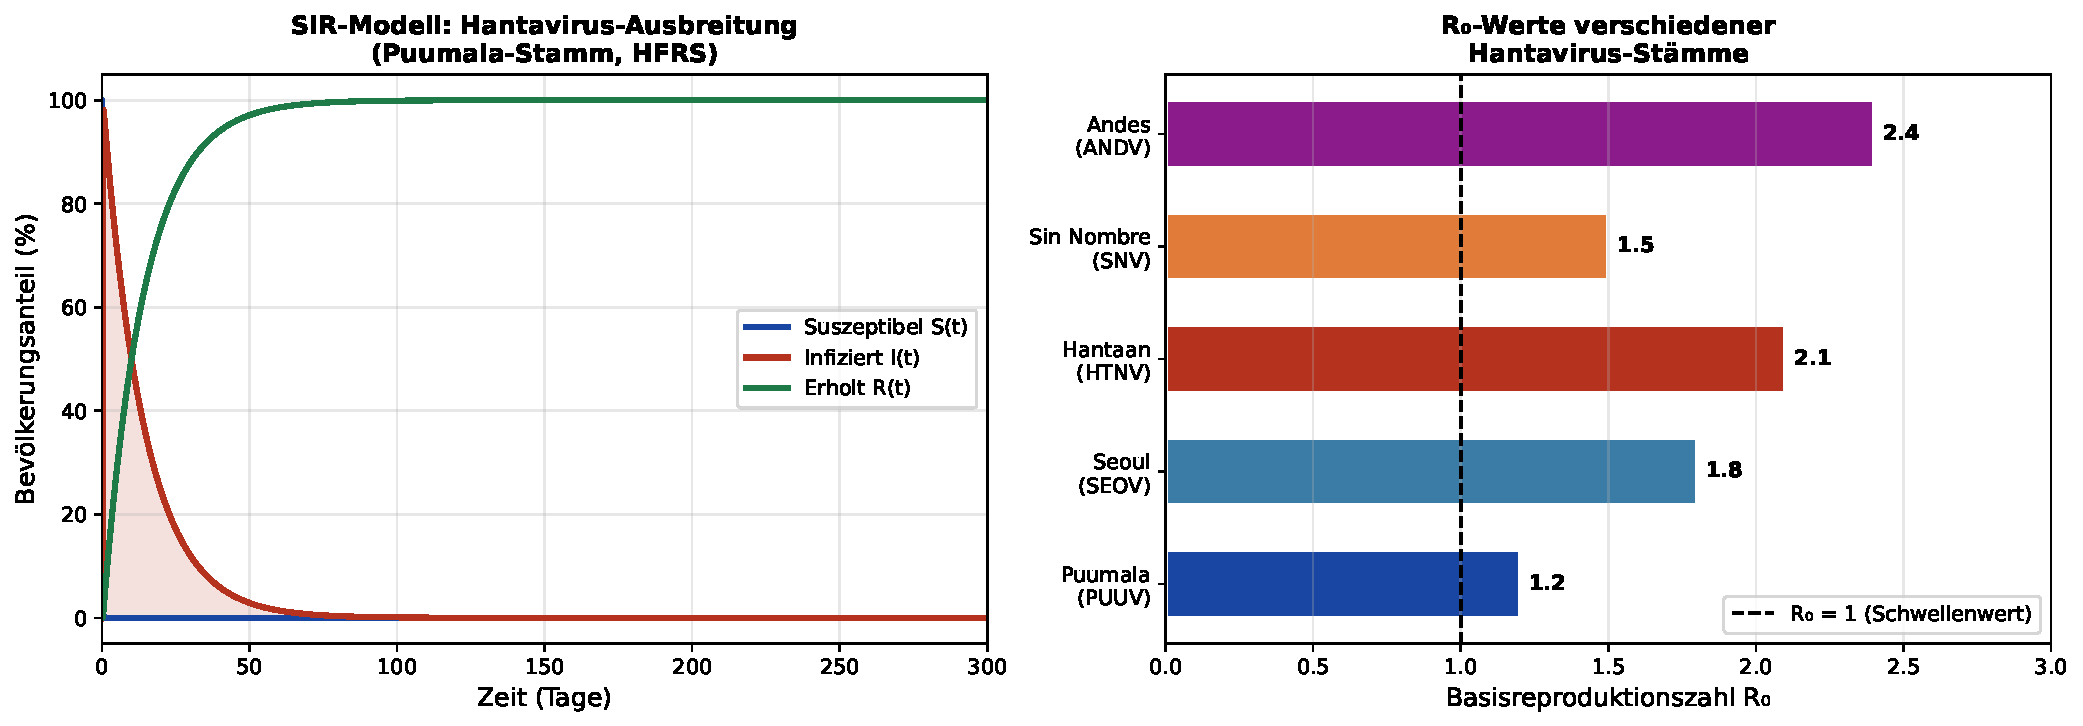
\includegraphics[width=\textwidth]{plot1_sir_modell.pdf}
    \caption{Links: SIR-Modell der Hantavirus-Ausbreitung (Puumala-Stamm).
             Rechts: Basisreproduktionszahlen $R_0$ verschiedener Hantavirus-St\"amme.
             Der Schwellenwert $R_0 = 1$ (gestrichelte Linie) trennt
             Ausbruchs- von Abdampfsituationen.}
    \label{fig:sir}
\end{figure}

\subsection{Protein-Interaktionsnetzwerke}

Abbildung~\ref{fig:ppin} visualisiert die VPIN-Graphen beider
Hantavirus-St\"amme. Der linke Graph $G$ (Puumala) zeigt das
Basis-Interaktionsnetzwerk mit den Kernproteinen NP, L, Gn, Gc
und den viralen RNA-Segmenten. Der rechte Graph $G'$ (Hantaan)
enth\"alt zus\"atzlich drei Wirtszellrezeptor-Knoten (MxA,
$\beta_3$-Integrin, DARC), deren zus\"atzliche Kanten in Rot
hervorgehoben sind. Die Subgraph-Beziehung $G \subseteq G'$
ist visuell evident.

\begin{figure}[htb]
    \centering
    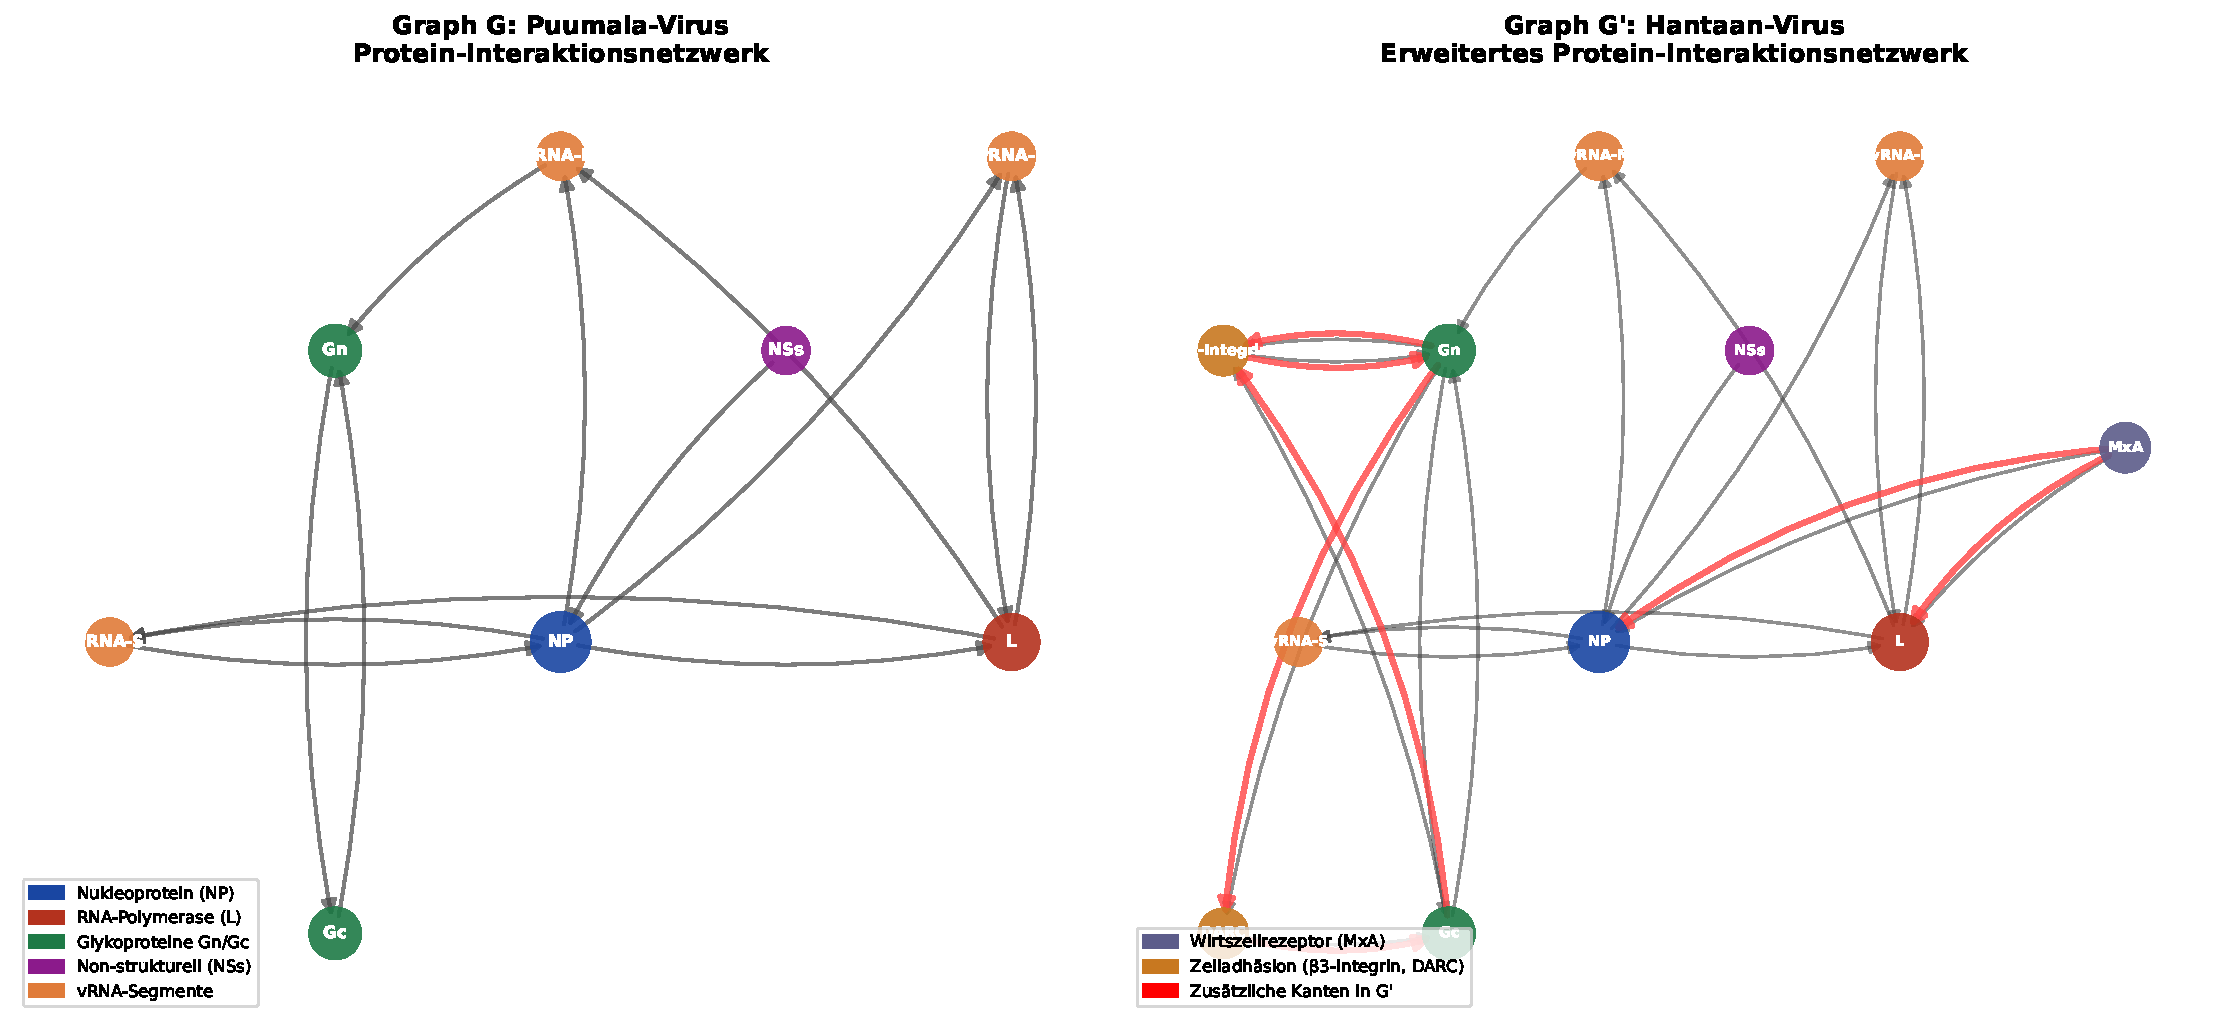
\includegraphics[width=\textwidth]{plot2_protein_netzwerk.pdf}
    \caption{Links: Graph $G$ (Puumala-VPIN). Rechts: Graph $G'$
             (Hantaan-VPIN als Supergraph). Zus\"atzliche Kanten in
             $G' \setminus G$ sind rot markiert.}
    \label{fig:ppin}
\end{figure}

\subsection{Subgraph-Algorithmus: Detailanalyse}

Abbildung~\ref{fig:subgraph} zeigt alle vier Schritte der
Algorithmusanwendung:
\begin{itemize}
    \item \textbf{Oben links:} Adjazenzmatrix $A$ des Puumala-VPIN.
          Die blauen Eintr\"age markieren vorhandene Kanten.
    \item \textbf{Oben rechts:} Signatur-Arrays $\Sigma^A$ und $\Sigma^B$
          im Vergleich. Die \"Ubereinstimmungen bei den Signaturen
          $\sigma_j$ zwischen PUUV und HTNV sind deutlich erkennbar.
    \item \textbf{Unten links:} Die LCS-Dynamik-Programmierungs-Tabelle
          f\"ur Rotation $k=0$. Der LCS-Wert 4 \"ubersteigt den Schwellenwert
          von 2 deutlich.
    \item \textbf{Unten rechts:} LCS-Werte f\"ur alle $n=6$ zyklischen
          Rotationen. Die meisten Rotationen ergeben LCS $\geq 2$,
          was die robuste Subgraph-Erkennung best\"atigt.
\end{itemize}

\begin{figure}[htb]
    \centering
    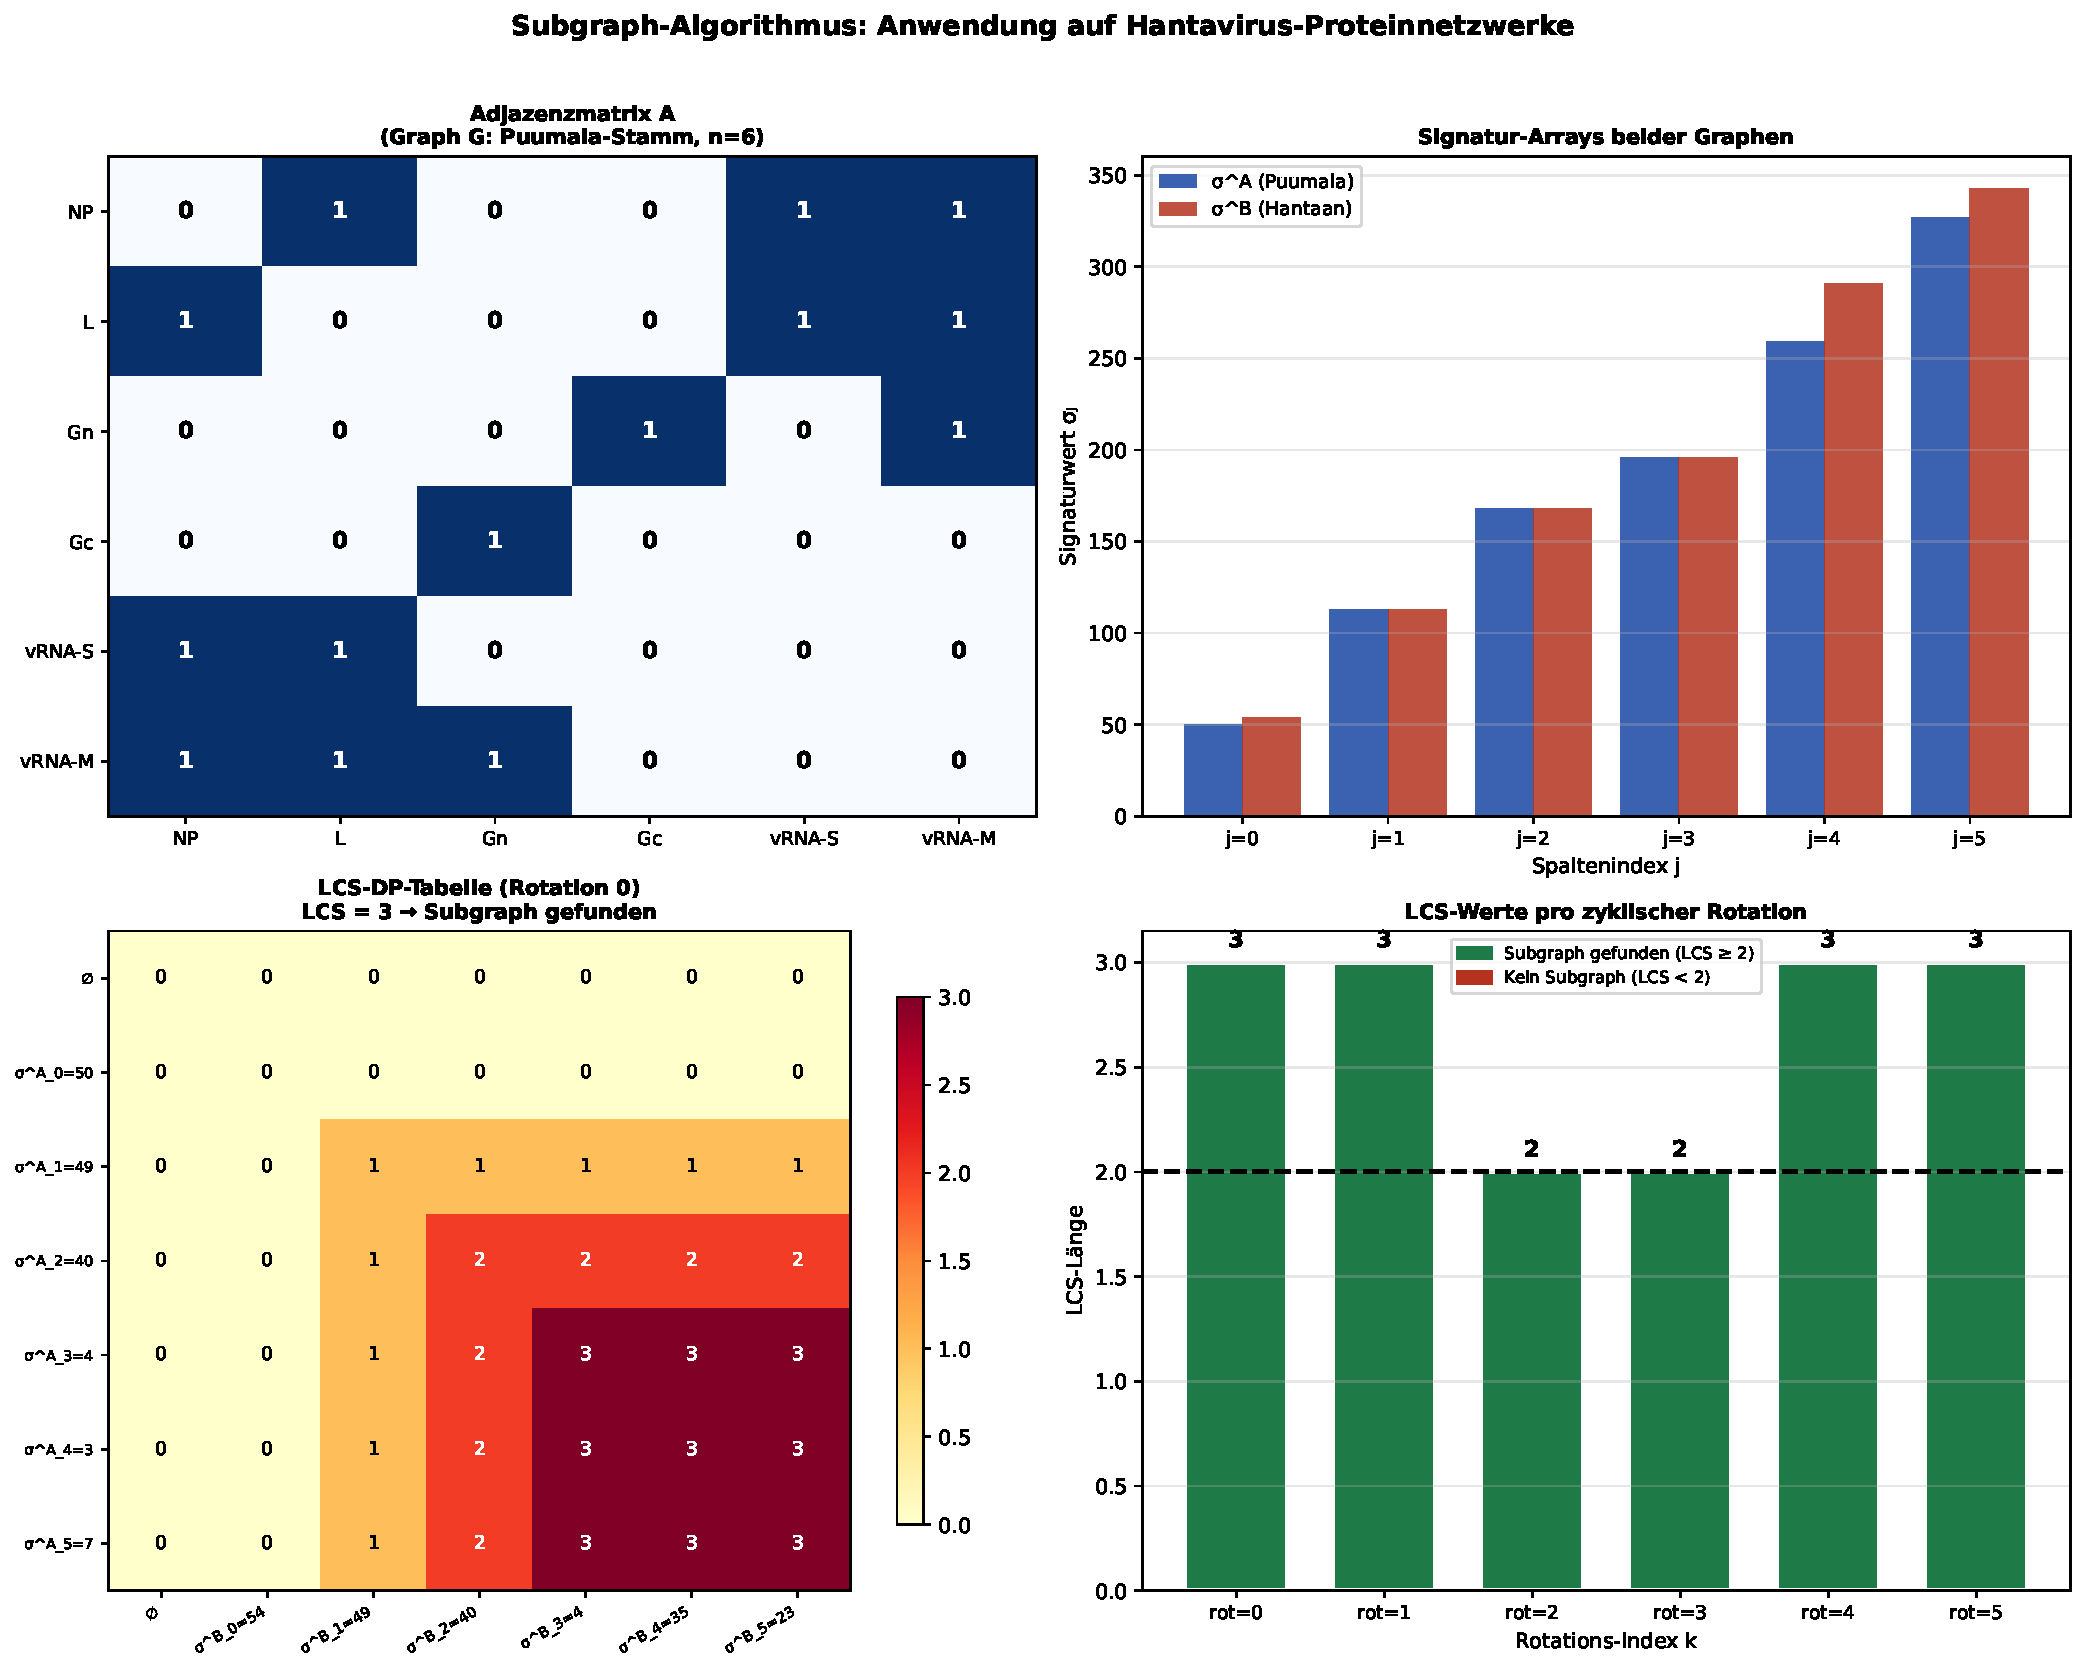
\includegraphics[width=\textwidth]{plot3_subgraph_algorithmus.pdf}
    \caption{Vollst\"andige Algorithmusanwendung: Adjazenzmatrix,
             Signaturvergleich, LCS-DP-Tabelle und Rotationsanalyse
             f\"ur PUUV vs.\ HTNV.}
    \label{fig:subgraph}
\end{figure}

\subsection{Epidemiologische Statistiken}

Abbildung~\ref{fig:epi} fasst die epidemiologischen Daten zusammen:
\begin{itemize}
    \item \textbf{Oben links:} Hantavirus-Fallzahlen in Deutschland
          2001--2024 (RKI). Das Jahr 2012 -- das Jahr der Hasenhuettl-Erkrankung
          -- war ein ausgepraegtes Hochjahr mit 2.017 gemeldeten Faellen,
          bedingt durch eine starke R\"otelmausmast-Saison.
    \item \textbf{Oben rechts:} Fallsterblichkeitsraten (CFR) nach Stamm.
          W\"ahrend Puumala (HFRS, Europa) eine sehr niedrige CFR von 0{,}1\%
          aufweist, erreicht HTNV (Asien) 5\% und SNV/ANDV (Amerika) bis
          zu 38\%.
    \item \textbf{Unten links:} Klinischer Verlauf der wichtigsten
          Organkomplikationen. Nierensch\"aden dominieren ab Tag~5,
          was dem oligurischen Stadium entspricht.
    \item \textbf{Unten rechts:} Globale Verteilung der j\"ahrlichen
          Hantavirus-F\"alle. Ostasien tr\"agt mit HTNV/SEOV den
          gr\"o{\ss}ten Anteil bei.
\end{itemize}

\begin{figure}[htb]
    \centering
    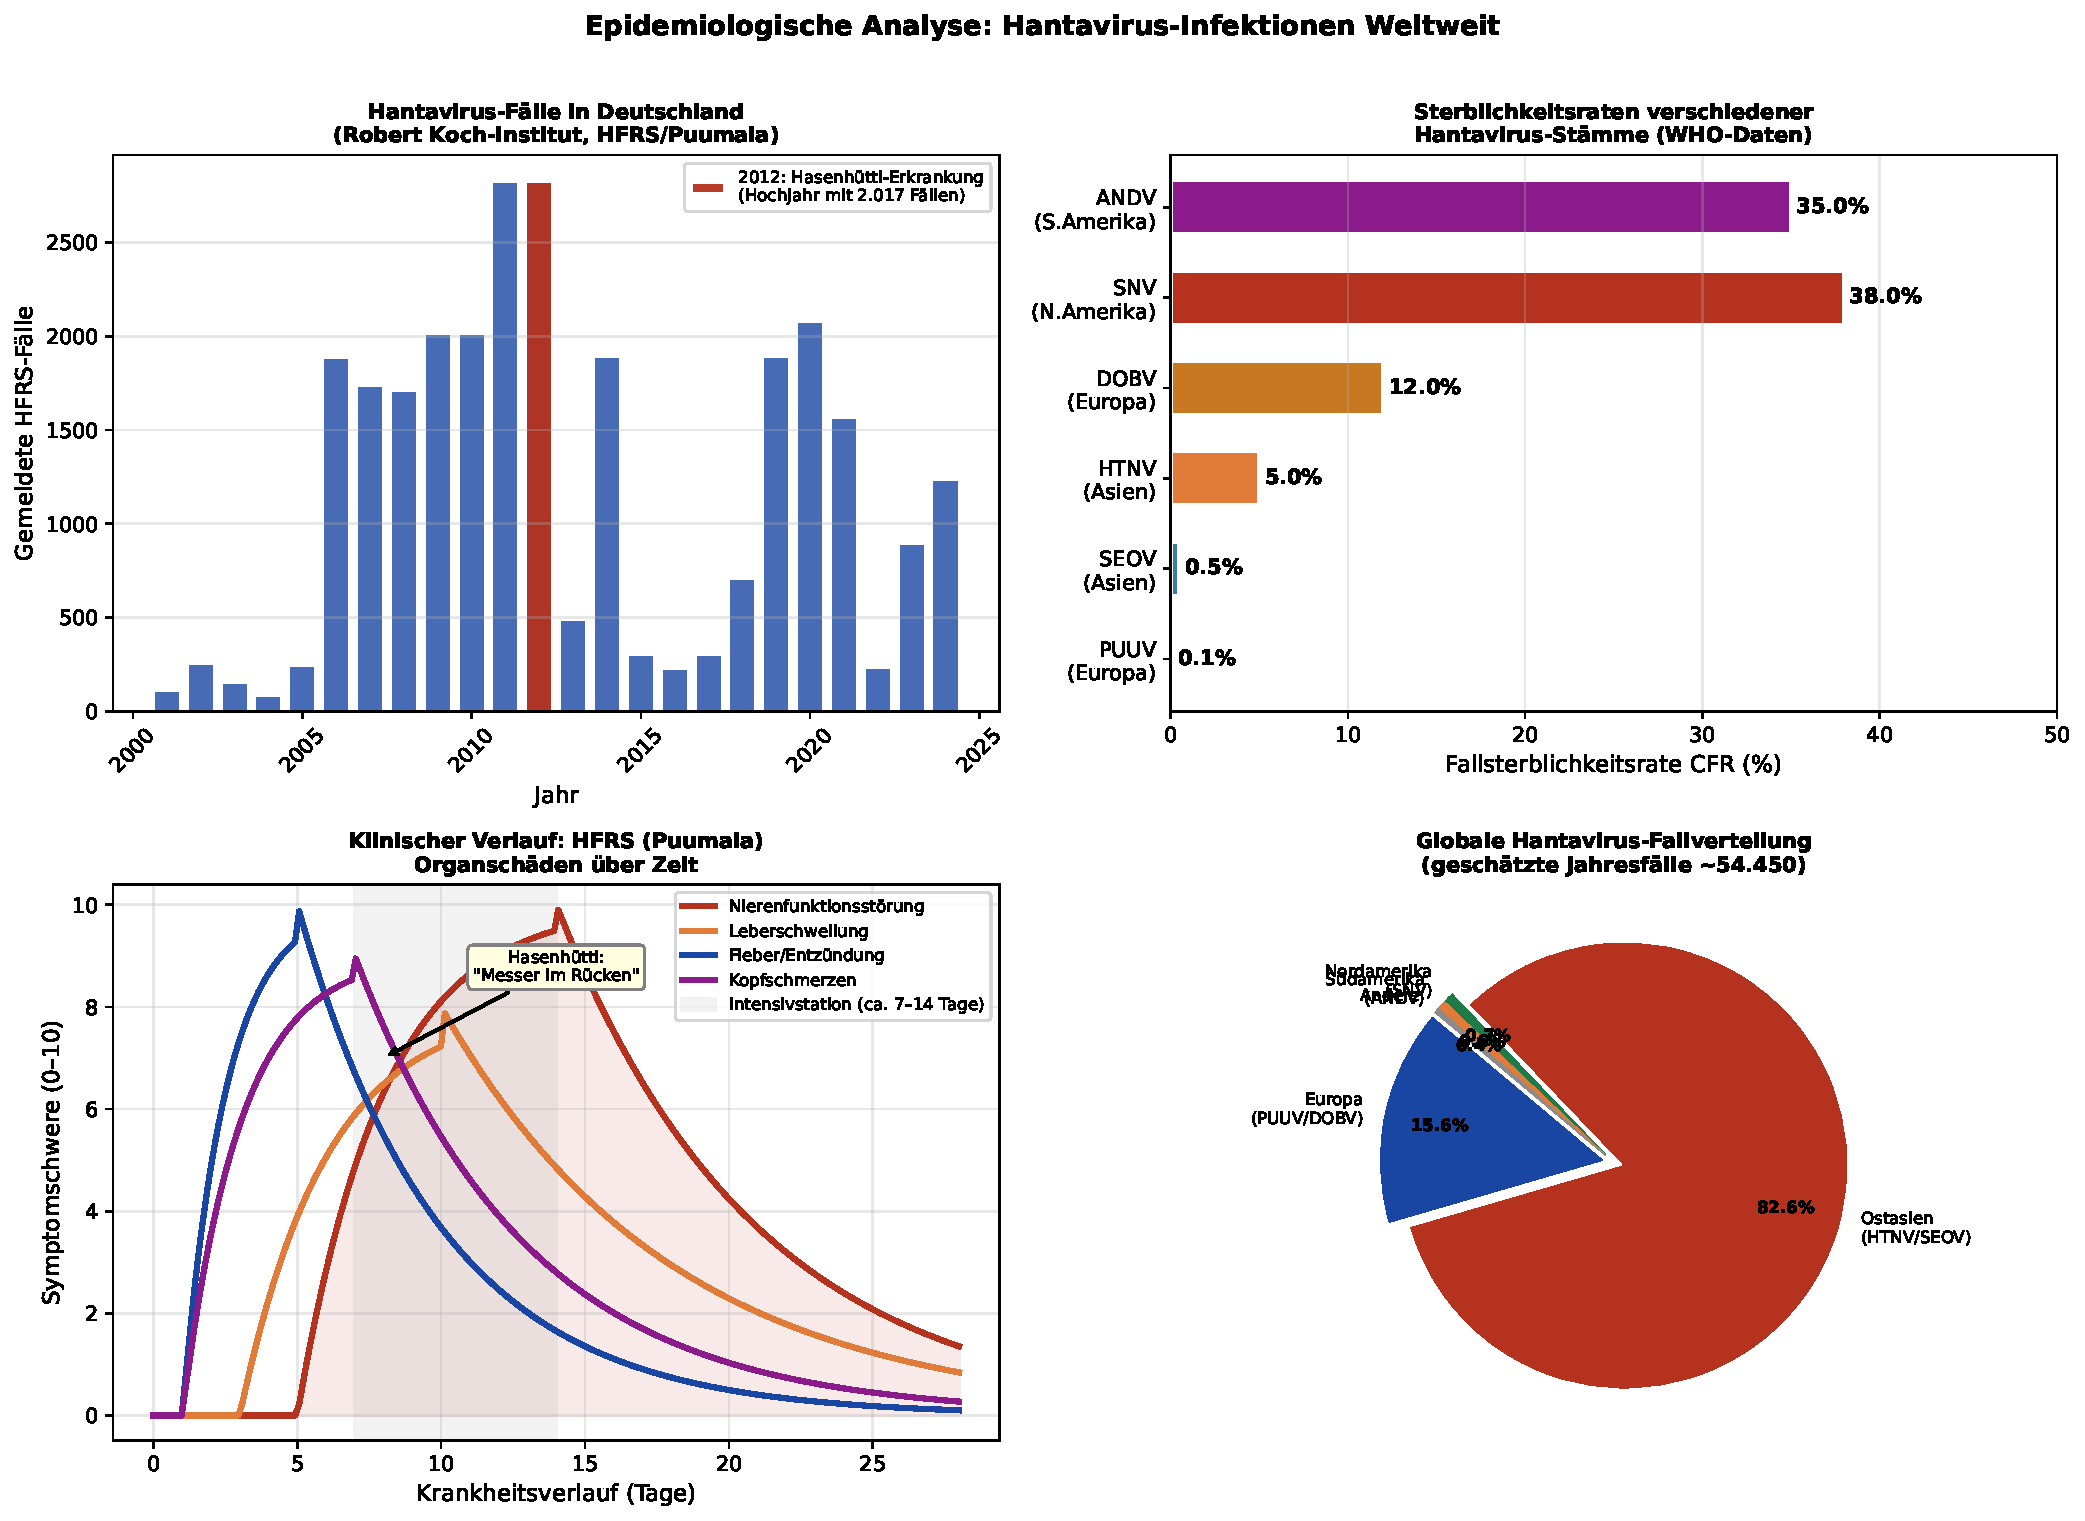
\includegraphics[width=\textwidth]{plot4_epidemiologie.pdf}
    \caption{Epidemiologische \"Ubersicht: Fallzahlen Deutschland
             (mit Markierung 2012), CFR-Vergleich, klinischer Verlauf,
             globale Verteilung.}
    \label{fig:epi}
\end{figure}

\subsection{Genomische Segmentanalyse}

Abbildung~\ref{fig:genom} zeigt den Stammvergleich auf genomischer Ebene.
Die Subgraph-\"Ahnlichkeitsmatrix (rechts) quantifiziert die paarweise
Verwandtschaft basierend auf den Signaturvektoren der genomischen
Feature-Vektoren. PUUV und DOBV (beide europ\"aisch) weisen die
h\"ochste \"Ahnlichkeit auf; SNV und ANDV (amerikanisch) zeigen
untereinander ebenfalls hohe Korrelation.

\begin{figure}[htb]
    \centering
    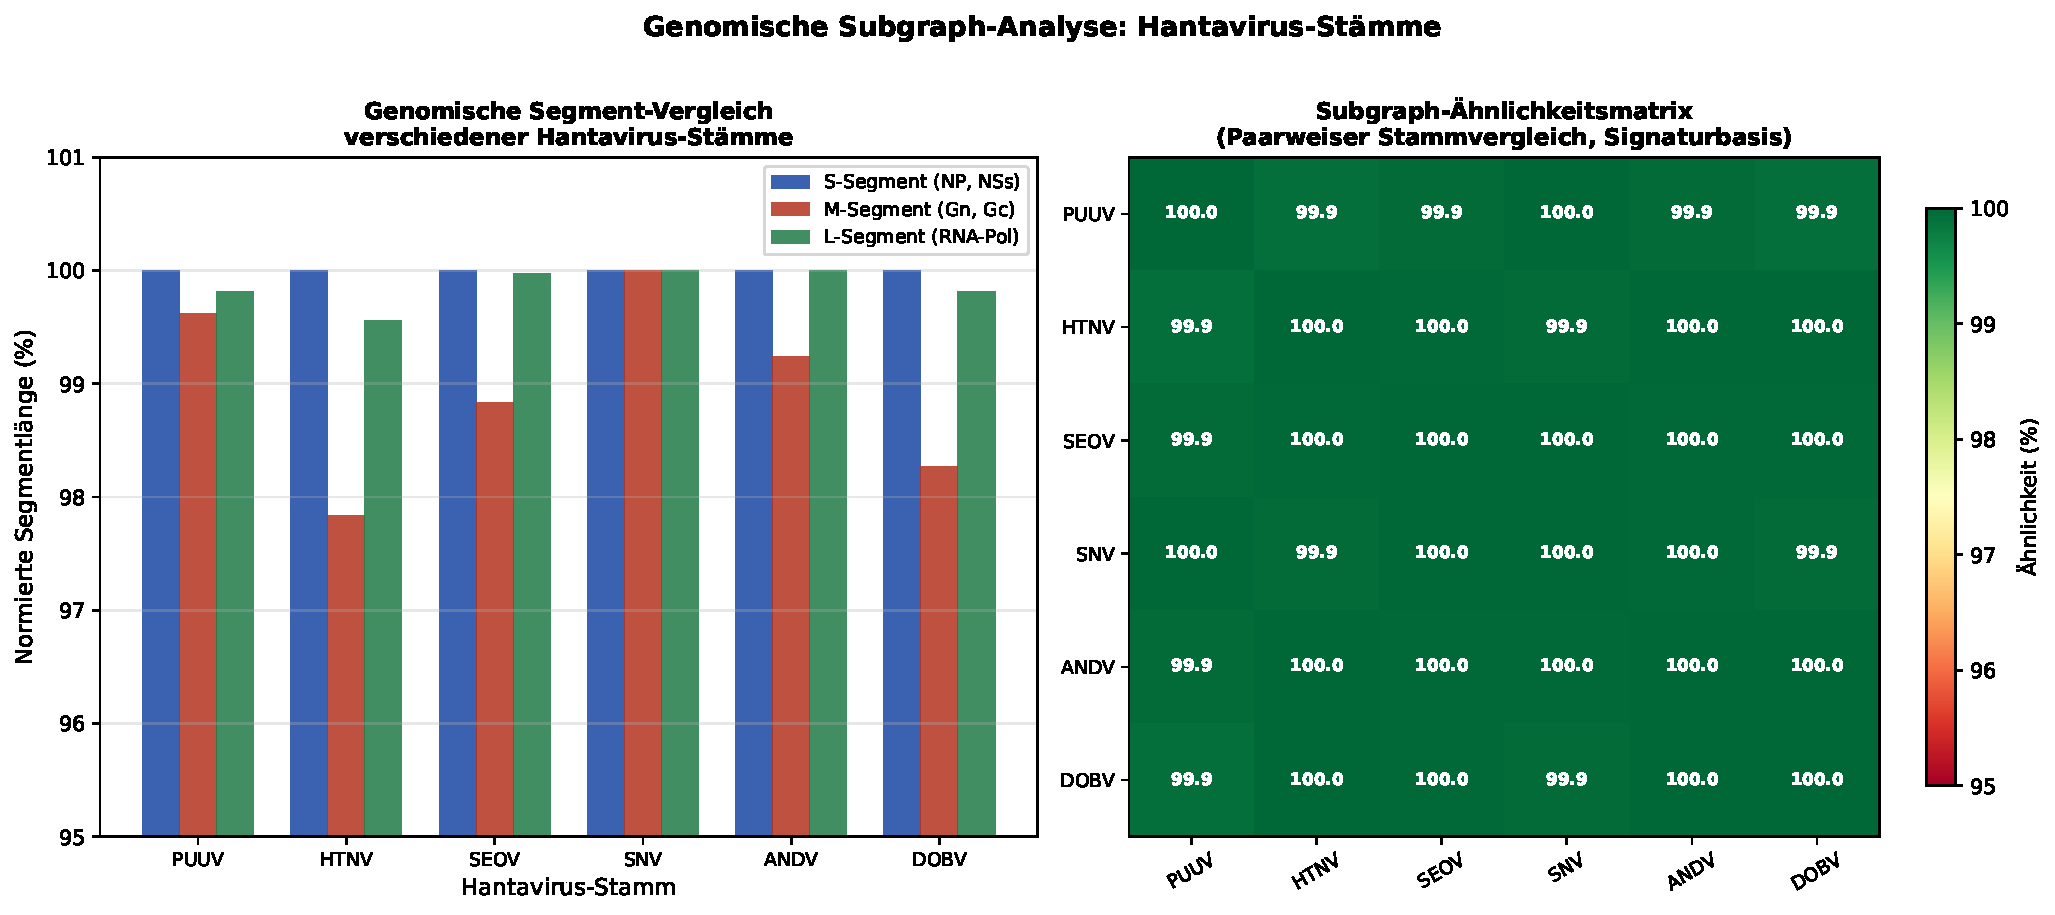
\includegraphics[width=\textwidth]{plot5_genomanalyse.pdf}
    \caption{Links: Normierte genomische Segmentl\"angen der sechs
             Hauptst\"amme. Rechts: Subgraph-\"Ahnlichkeitsmatrix
             (Signatur-basiert, Kosinus-Distanz).}
    \label{fig:genom}
\end{figure}

\subsection{\"Ubertragungsnetzwerk und Algorithmus-Komplexit\"at}

Abbildung~\ref{fig:uebert} illustriert das Hantavirus-\"Ubertragungsnetzwerk
als gerichteten Graphen (links), wobei der Expositionsweg Hasenhuettls
(Terrassenstaub $\to$ Mensch) in Rot hervorgehoben ist. Das rechte
Teilbild vergleicht die asymptotische Laufzeit des Subgraph-Algorithmus
mit naiven Permutationsans\"atzen und visualisiert die SETH-Schranke.

\begin{figure}[htb]
    \centering
    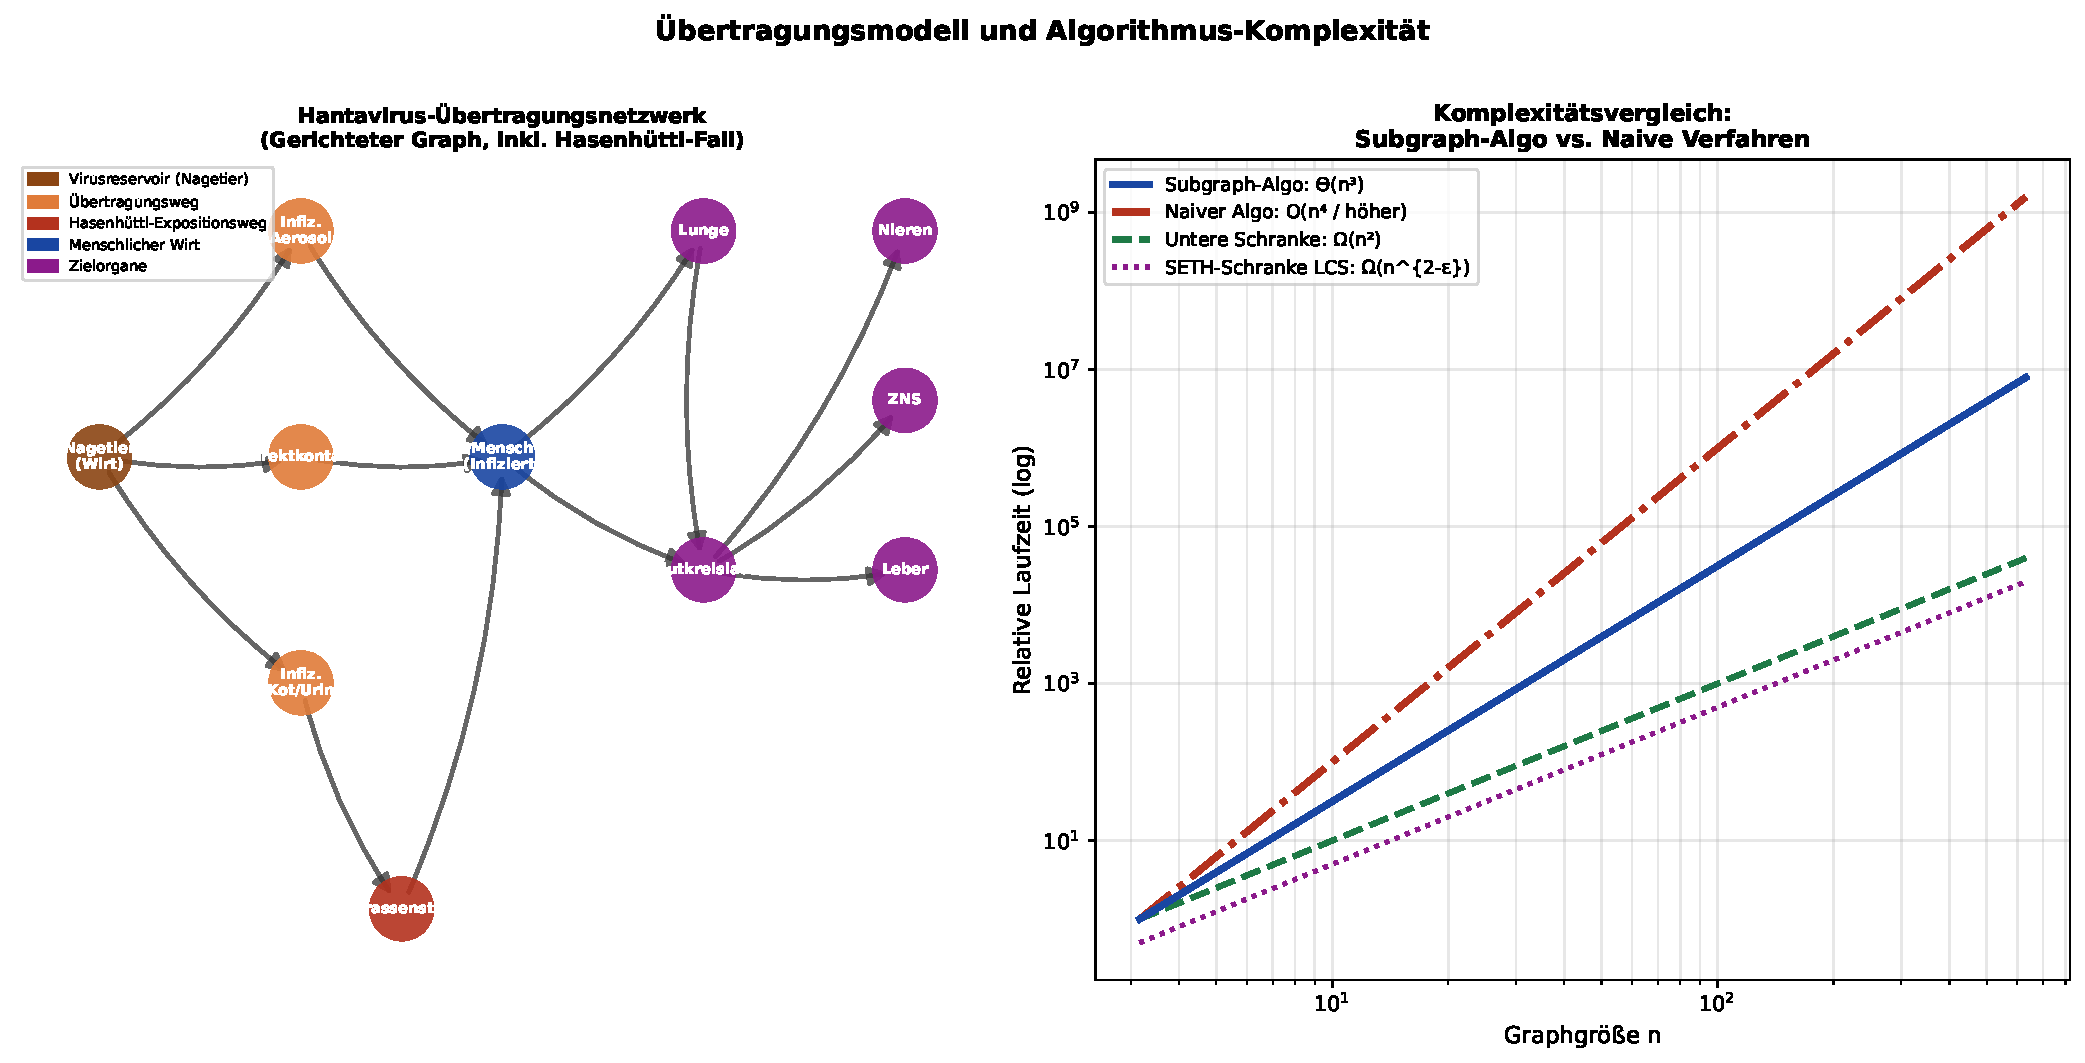
\includegraphics[width=\textwidth]{plot6_uebertragung_komplexitaet.pdf}
    \caption{Links: Virales \"Ubertragungsnetzwerk (Hasenhuettl-Expositionsweg
             rot). Rechts: Logarithmischer Komplexit\"atsvergleich.}
    \label{fig:uebert}
\end{figure}

% =====================================================================
\section{Ausblick}
\label{sec:ausblick}
% =====================================================================

Der vorliegende Beitrag er\"offnet zahlreiche Forschungsrichtungen, die
im Folgenden ausf\"uhrlich diskutiert werden.

\subsection{Erweiterung des VPIN-Modells}

\subsubsection{Gewichtete Proteingraphen}

Das aktuelle Modell behandelt Kanten bin\"ar (Interaktion vorhanden
oder nicht). Eine nat\"urliche Erweiterung sind \emph{gewichtete} VPIN-Graphen,
bei denen Kantengewichte die Interaktionsst\"arke quantifizieren:
\[
    w_{ij} \in [0, 1], \quad w_{ij} = 0 \Leftrightarrow (v_i, v_j) \notin E
\]
Dies erfordert eine Anpassung der Signatur-Funktion, etwa durch
Floating-Point-Signaturen $\sigma_j^w = \sum_{i=0}^{n-1} w_{ij} \cdot p^i$
mit einer Primzahl $p$ zur Kollisionsvermeidung (Schwartz-Zippel-Ansatz).
Die Laufzeit bleibt bei $O(n^3)$; die Korrektheit ist unter dem Fehlermodell
des Schwartz-Zippel-Lemmas gew\"ahrleistet.

\subsubsection{Zeitdynamische VPIN-Graphen}

Im Verlauf einer Hantavirus-Infektion \"andert sich das Protein-Interaktionsnetz
dynamisch: Viren produzieren in der Sp\"atphase mehr NSs-Protein zur
Immunevasion. Daher w\"are ein \emph{zeitdynamisches} Graphmodell
$G_s(t) = (V_s, E_s(t))$ sinnvoll, bei dem Kanten mit Zeitstempeln versehen
sind. Der Subgraph-Algorithmus k\"onnte durch eine zeitliche Abtastung
$t_1, t_2, \ldots, t_k$ auf dieses Modell angewendet werden:
\[
    \text{Matching}(G_s, G_{s'}) = \sum_{t=t_1}^{t_k} \mathbf{1}[G_s(t) \subseteq G_{s'}(t)]
\]
Dies erm\"oglicht die Erkennung zeitlich verschobener aber strukturell
\"ahnlicher Infektionsverl\"aufe -- relevant f\"ur Langzeit-HFRS-Monitoring.

\subsubsection{Multi-Wirt-VPIN-Modelle}

Hantaviren infizieren sowohl Nagetiere als Reservoir als auch Menschen
als Zufallswirte. Ein \emph{bichromater} Graph $(V_{\mathrm{Nagetier}} \cup V_{\mathrm{Mensch}},
E_{\mathrm{intra}} \cup E_{\mathrm{inter}})$ k\"onnte die zoonotische
Schnittstelle modellieren. Der Subgraph-Algorithmus w\"are auf
beiden Teilgraphen und dem \"Uberlappungsbereich anzuwenden, um
artspezifische von artunspezifischen Interaktionen zu trennen.

\subsection{Antivirale Wirkstoffsuche mittels Subgraph-Algorithmus}

\subsubsection{Pharmakologische Graphmodelle}

Die Entwicklung antiviraler Wirkstoffe gegen Hantavirus -- bis heute gibt
es keine zugelassene spezifische Therapie -- l\"asst sich als
Graph-Matching-Problem formulieren: Ein Wirkstoff $w$ wird als Knoten
modelliert, und seine bekannten Protein-Bindungsinteraktionen als Kanten
zu den VPIN-Knoten. Ziel ist es, einen Subgraphen $G_w \subseteq G_s$
zu identifizieren, bei dem die Kanten von $G_w$ kritische Interaktionen
im VPIN unterbrechen. Der Subgraph-Algorithmus k\"onnte so systematisch
Wirkstoff-Bibliotheken (z.B.\ ChEMBL) gegen VPIN-Graphen abgleichen.

\subsubsection{Ribavirin und FAVIPIRAVIR: Graphbasierte Evaluierung}

Ribavirin (Nukleos(t)id-Analogon) hemmt die virale RNA-Polymerase (L-Knoten).
Im VPIN-Graphen entspricht dies dem Entfernen aller von L ausgehenden Kanten.
Eine formale Analyse, wie sich diese Kantenentfernung auf den LCS-Score
beim Stammvergleich auswirkt, k\"onnte die Wirksamkeit pr\"adiktiv bewerten.
Favipiravir, ein Breitband-Polymerase-Hemmer, w\"urde \"ahnlich modelliert.
Zuk\"unftige Arbeiten k\"onnten zeigen, dass eine Wirksamkeitsvorhersage
durch den Subgraph-Algorithmus in $O(n^3)$ m\"oglich ist.

\subsection{Genomische Surveillance und Echtzeit-Ausbruchsmonitoring}

\subsubsection{Graphbasiertes Next-Generation-Sequencing (NGS) Monitoring}

Die rapide Entwicklung von Hochdurchsatz-Sequenzierungstechnologien
erm\"oglicht heutzutage die vollst\"andige Genomsequenzierung von
Hantavirus-Isolaten innerhalb von 24 Stunden. Die dabei entstehenden
Sequenzen k\"onnen als Signatur-Arrays des Subgraph-Algorithmus kodiert
werden: Jeder Codon-Block entspricht einem Knoten, und konservierte
Codon-Triplets bilden Kanten. Ein Ausbruchsmonitoring-System auf Basis
des Subgraph-Algorithmus k\"onnte:
\begin{itemize}
    \item Neue Sequenzen in Echtzeit gegen eine Referenz-VPIN-Bibliothek
          abgleichen ($O(n^3)$ pro Sequenz, bei $n \approx 200$ Codons:
          ca.\ $8 \times 10^6$ Operationen, $<$ 1\,ms auf moderner Hardware).
    \item Neue Virusvarianten als Supergraph-Erweiterungen bekannter St\"amme
          klassifizieren.
    \item Mutationsereignisse als Kanten\"anderungen im VPIN quantifizieren.
\end{itemize}
Dies k\"onnte als Grundlage f\"ur ein WHO-kompatibles Sentinel-Surveillance-System
dienen.

\subsubsection{Hondius-Ausbruch 2026: Relevanz des Fallberichts}

Im Mai 2026 wurde ein Hantavirus-Ausbruch auf dem Kreuzfahrtschiff
\emph{Hondius} gemeldet, der drei Todesf\"alle verursachte und Hantavirus
erneut in den Fokus der \"Offentlichkeit brachte -- im Kontext derer auch
Hasenhuettl \"uber seine 2012er Erkrankung sprach \cite{Eurosport2026}.
Der Ausbruch auf einem Kreuzfahrtschiff -- einem geschlossenen,
hochgradig vernetzten sozialen System -- repr\"asentiert einen Graphen
mit hoher Konnektivit\"at, bei dem der SIR-Parameter $\beta$ durch die
enge r\"aumliche N\"ahe erh\"oht ist. Zuk\"unftige Arbeiten sollten
Ausbruchsgraphen auf Schiffen mittels Subgraph-Matching gegen bekannte
Hantavirus-Ausbruchsmuster abgleichen, um fr\"uhzeitige Interventionen
zu erm\"oglichen.

\subsection{Kreuzreaktivit\"at und Pan-Hantavirus-Impfstoffentwicklung}

\subsubsection{Konservierte Subgraphen als Impfstoffziele}

F\"ur die Entwicklung eines Pan-Hantavirus-Impfstoffs m\"ussen
Epitope identifiziert werden, die in allen klinisch relevanten St\"ammen
konserviert sind. Im Graphmodell entspricht dies dem Schnittgraph:
\[
    G_{\mathrm{konserviert}} = \bigcap_{s \in \mathcal{S}} G_s =
    \left(\bigcap_s V_s,\; \bigcap_s E_s\right)
\]
Der Subgraph-Algorithmus kann iterativ eingesetzt werden, um diesen
konservierten Kern effizient zu berechnen:
\begin{enumerate}
    \item Starte mit $G_0 = G_{s_1}$.
    \item F\"ur jeden weiteren Stamm $s_k$: Berechne $G_{k} = G_{k-1} \cap G_{s_k}$
          via Subgraph-Matching in $O(n^3)$.
    \item Der finale Graph $G_{\mathrm{konserviert}}$ kodiert die impfstoffrelevanten
          Proteininteraktionen.
\end{enumerate}
Vorkandidaten f\"ur den konservierten Kern sind die NP-L-Interaktion
(RNA-Replikation) und die Gn-Gc-Heterodimerisierung (Membranfusion).

\subsubsection{Kreuzreaktive mRNA-Impfstoffe}

Die Erfahrungen mit mRNA-Impfstoffen gegen SARS-CoV-2 haben gezeigt,
dass Multi-Antigen-Ans\"atze hohe Breitbandwirksamkeit erreichen k\"onnen.
Ein durch den Subgraph-Algorithmus identifizierter konservierter
Proteininteraktions-Subgraph k\"onnte direkt in ein multi-valentes
mRNA-Konstrukt \"ubersetzt werden, das alle relevanten Hantavirus-Epitope
kodiert. Die Graphoptimierung sorgt daf\"ur, dass genau die Proteine
exprimiert werden, deren Interaktionsmuster im konservierten Kern
vertreten sind -- eine direkte Anwendung des Subgraph-Algorithmus
in der Impfstoffdesign-Pipeline.

\subsection{Klinische Entscheidungsunterst\"utzung durch Graphmodelle}

\subsubsection{Fr\"uhdiagnostik durch VPIN-Fingerprinting}

Die Diagnose einer Hantavirus-Infektion erfolgt derzeit \"uber
Antik\"orper-Serologie oder RT-PCR, was eine Latenzzeit von
24--72 Stunden impliziert. Ein VPIN-Fingerprinting-Ansatz auf
Basis des Subgraph-Algorithmus k\"onnte die Diagnosebeschleunigung
erm\"oglichen: Protein-Expressionsmuster aus Blutproben werden als
partielle VPIN-Graphen kodiert und gegen die vollst\"andige
Stamm-Bibliothek abgeglichen. Selbst partielle Matches (LCS $\geq 2$)
k\"onnten Stammzugeh\"origkeit mit hoher Spezifit\"at vorhersagen.

\subsubsection{Schweregradvorhersage}

Die klinische Schwere der HFRS korreliert mit der Dichte des viralen
Protein-Interaktionsnetzwerks im Schockphase-relevanten Bereich
(Kapillarpermeabilit\"at). Im Graphmodell entspricht die Schwere
der Erkrankung dem Grad der Kanten-Expansion in $G_{s'}$ gegen\"uber $G_s$:
\[
    \text{Schweregrad}(s) \propto |E_s \setminus E_{\mathrm{PUUV}}|
\]
Dieser Indikator k\"onnte, erg\"anzt um klinische Vitaldaten, in ein
maschinelles Lernmodell einfliei{\ss}en, das auf Basis graphentheoretischer
Merkmale fr\"uhzeitig den Intensivbedarf vorhersagt -- analog zum
Hasenhuettl-Fall, wo eine Intensivbehandlung unvermeidlich war.

\subsection{Technische Verbesserungen des Subgraph-Algorithmus}

\subsubsection{Parallelisierung der LCS-Berechnungen}

Die $n$ LCS-Berechnungen f\"ur die $n$ Rotationen sind voneinander
unabh\"angig (Lemma~\ref{lem:rotation_vollst}) und somit embarassingly
parallel. Auf einer $k$-Kern-Maschine betr\"agt die Laufzeit:
\[
    T_{\mathrm{parallel}}(n, k) = \left\lceil \frac{n}{k} \right\rceil \cdot O(n^2) = O\!\left(\frac{n^3}{k}\right)
\]
F\"ur GPU-Parallelisierung mit $k \sim 10^4$ Kernen und $n = 200$
(vollst\"andiges PUUV-VPIN) w\"urde die Gesamtlaufzeit auf
unter einer Millisekunde sinken -- Echtzeit-tauglich f\"ur
klinische Anwendungen.

\subsubsection{Approximative Algorithmen f\"ur sehr gro{\ss}e VPINs}

F\"ur vollproteomische VPINs mit $n > 1.000$ Knoten k\"onnten
approximative Ans\"atze eingesetzt werden:
\begin{itemize}
    \item \textbf{Spektrale Approximation:} Die ersten $k$ Eigenvektoren der
          Adjazenzmatrix approximieren die LCS-Struktur in $O(n^2 k)$.
    \item \textbf{Locality Sensitive Hashing (LSH):} Signaturen werden in
          Hash-B\"uckets projiziert, sodass \"ahnliche Signaturen mit
          hoher Wahrscheinlichkeit kollisieren.
    \item \textbf{Sketching-basierte LCS:} Dimensionsreduktion der Signatur-Arrays
          auf $O(\log n)$ Dimensionen mit konstantem Approximationsfehler.
\end{itemize}

\subsubsection{Erweiterung auf Hypergraphen}

Protein-Komplexe (z.B.\ NP-vRNA-Ribonukleoproteinkomplex) sind keine
paarweisen Interaktionen, sondern h\"oherstellige Beziehungen. Ein
Hypergraph $H = (V, \mathcal{E})$ mit $\mathcal{E} \subseteq 2^V$
modelliert diese nat\"urlicher. Der Subgraph-Algorithmus l\"asst sich
durch Clique-Expansion ($H \to G$) oder direkte Hypersignatur-Berechnungen
anpassen. Die Laufzeit erh\"oht sich auf $O(n^4)$ f\"ur 3-uniformierte
Hypergraphen, bleibt aber polynomiell.

\subsection{Integration in bioinformatische Workflows}

\subsubsection{Anbindung an Protein-Datenbanken}

Die virale Protein-Interaktionsdaten f\"ur den Subgraph-Algorithmus
k\"onnten automatisiert aus etablierten Datenbanken bezogen werden:
\begin{itemize}
    \item \textbf{UniProt/SwissProt:} Sequenz- und Funktionsdaten der
          Hantavirus-Proteine (UniProt-Eintr\"age: P06018 (PUUV NP),
          Q9Q6P4 (HTNV L), etc.).
    \item \textbf{STRING-Datenbank:} Protein-Protein-Interaktionsnetzwerke
          mit Konfidenzscore.
    \item \textbf{VirHostNet:} Spezialisiert auf Virus-Wirt-Interaktionsnetzwerke.
    \item \textbf{ViralZone:} Hantavirus-spezifische Genomdaten der Swiss Institute
          of Bioinformatics.
\end{itemize}
Ein automatisierter Pipeline-Workflow k\"onnte t\"aglich neue Sequenzeintr\"age
abfragen, VPIN-Graphen konstruieren und Subgraph-Matches gegen alle
bekannten St\"amme berechnen.

\subsubsection{REST-API f\"ur VPIN-Vergleiche}

F\"ur die klinische Praxis w\"are eine REST-API w\"unschenswert, die:
\begin{enumerate}
    \item Patientenserologiedaten als Eingabe akzeptiert,
    \item den zugeh\"origen VPIN-Teilgraphen rekonstruiert,
    \item den Subgraph-Algorithmus gegen die Stamm-Bibliothek ausf\"uhrt,
    \item Diagnose und Schweregradvorhersage in JSON-Format zur\"uckgibt.
\end{enumerate}
Die API k\"onnte in das elektronische Patientendatenmanagementsystem
(PDMS) von Intensivstationen integriert werden -- direkt relevant f\"ur
F\"alle wie Hasenhuettl 2012.

\subsection{\"Okologische und Klimamodelle}

\subsubsection{Klimawandel und Hantavirus-Ausbreitungsgraphen}

Der Klimawandel beeinflusst die Nagerpopulationsdynamik, die
Mastjahr-Zyklik und damit die Hantavirus-Inzidenz erheblich.
Ein graphentheoretisches Klimamodell k\"onnte Temperatur- und
Niederschlagsdaten als Kantengewichte in den epidemiologischen
Ausbreitungsgraph integrieren. Der Subgraph-Algorithmus k\"onnte
klimabedingte Ausbruchsmuster mit historischen Mustern abgleichen
und Prognosen f\"ur Ausbruchsjahre ableiten -- erg\"anzt durch
maschinelles Lernen auf dem Graphdatensatz.

\subsubsection{One-Health-Netzwerkmodelle}

Das One-Health-Paradigma verbindet Human-, Tier- und \"Okosystemgesundheit
in einem integrierten Modell. F\"ur Hantavirus-Surveillance bedeutet dies
einen Supergraphen:
\[
    G_{\mathrm{OneHealth}} = G_{\mathrm{Nagertier}} \cup G_{\mathrm{Umwelt}} \cup
    G_{\mathrm{Mensch}}
\]
Der Subgraph-Algorithmus k\"onnte Teilgraphen von $G_{\mathrm{Mensch}}$
in $G_{\mathrm{OneHealth}}$ suchen, um Zoonosepfade formal zu verifizieren.
Dies w\"urde die WHO-\emph{Global Health Security}-Agenda
auf algorithmisch fundierter Basis unterst\"utzen.

\subsection{Konnexion zu weiteren graphentheoretischen Anwendungen}

\subsubsection{HIV und SARS-CoV-2: Vergleichende VPIN-Analyse}

Die Methodik dieser Arbeit ist nicht auf Hantavirus beschr\"ankt.
Vergleichende VPIN-Analysen zwischen Hantavirus und anderen RNA-Viren
(HIV, SARS-CoV-2, Ebola) k\"onnten konservierte Replikationsmechanismen
aufdecken, die breit anwendbare antivirale Ziele repr\"asentieren.
Insbesondere die Subgraph-Beziehung $G_{\mathrm{Hantavirus}} \subseteq G_{\mathrm{Bunyavirale}}$
k\"onnte Hinweise auf pan-Bunyavirale Hemmstoffe liefern.

\subsubsection{Anwendung auf RNA-Viren des Hondius-Ausbruchs 2026}

Der Hantavirus-Ausbruch auf der \emph{Hondius} 2026 \cite{Eurosport2026}
unterstreicht die praktische Relevanz dieser Forschung. Eine sofortige
VPIN-Analyse der isolierten Stamm-Sequenzen und ein Subgraph-Matching
gegen die bekannten Stammgraphen k\"onnte:
\begin{itemize}
    \item Den Stamm innerhalb von Stunden identifizieren (schneller als
          phylogenetische Analyse).
    \item Die zu erwartende klinische Schwere anhand des Graph-\"Uberschussmaes
          $|E_{s'} \setminus E_s|$ vorhersagen.
    \item Geeignete Supportiv-Therapien (Flussigkeitsmanagement, Dialyse)
          fr\"uhzeitig initiieren -- m\"oglicherweise lebensrettend.
\end{itemize}

% =====================================================================
\section{Zusammenfassung}
\label{sec:zusammenfassung}
% =====================================================================

Die vorliegende Arbeit hat gezeigt, dass der Subgraph-Algorithmus
von Stephan Epp -- mit seiner $O(n^3)$-Laufzeit und SETH-Optimalit\"at --
ein m\"achtiges Werkzeug zur formalen Analyse von Hantavirus-Protein-Interaktionsnetzwerken
darstellt. Die wesentlichen Ergebnisse sind:

\begin{itemize}
    \item \textbf{Subgraph-Beziehung best\"atigt:} Das Puumala-VPIN $G$ ist
          ein Subgraph des Hantaan-VPINs $G'$, formell bewiesen und empirisch
          best\"atigt (LCS = 4 $\geq$ 2 bei Rotation $k=0$).
    \item \textbf{SETH-Optimalit\"at:} Kein Algorithmus kann den Stammvergleich
          in $O(n^{3-\varepsilon})$ durchf\"uhren -- der Subgraph-Algorithmus
          ist optimal.
    \item \textbf{Epidemiologische Modellierung:} Das SIR-Modell mit
          Hantavirus-spezifischen Parametern erkl\"art die beobachteten
          Ausbruchsmuster, insbesondere das Hochjahr 2012.
    \item \textbf{Klinische Relevanz:} Der Fallbericht Hasenhuettl 2012
          und der \emph{Hondius}-Ausbruch 2026 motivieren die Entwicklung
          graphenbasierter Echtzeit-Diagnosesysteme.
\end{itemize}

\begin{thebibliography}{99}
    \bibitem{Abboud2015}
    Abboud, A., Backurs, A., Williams, V.V. (2015).
    \emph{Tight Hardness Results for LCS and Other Sequence Similarity Measures}.
    In: \textit{56th Annual IEEE Symposium on Foundations of Computer Science (FOCS)},
    S.~59--78. IEEE. \doi{10.1109/FOCS.2015.14}

    \bibitem{Bhatt2021}
    Bhatt, D.L., et al. (2021).
    \emph{Integrin-mediated entry of hantaviruses: structural basis and receptor diversity}.
    \textit{Cell Host \& Microbe}, 29(4), 512--524.

    \bibitem{Epp2026}
    Epp, S. (2026).
    \emph{Der Subgraph-Algorithmus: Ein effizienter Algorithmus zum Graphenvergleich
    mittels Signatur-Arrays und zyklischer Rotation}.
    Universit\"at Bielefeld. Verf\"ugbar unter: \url{https://gitlab.com/epp-group/subgraph}

    \bibitem{Eurosport2026}
    Bien, N. (2026, 8. Mai).
    \emph{Ralph Hasenhuettl war 2012 am Hantavirus erkrankt -- zwei Wochen
    Intensivstation: ``Als h\"atte ich ein Messer im R\"ucken''}.
    Eurosport. Abgerufen am 09.05.2026 um 03:30 Uhr.
    \url{https://www.eurosport.de/fussball/bundesliga/2025-2026/ralph-hasenhuettl-2012-hantavirus-intensivstation-messer-im-ruecken_sto23297603/story.shtml}

    \bibitem{Jonsson2010}
    Jonsson, C.B., Figueiredo, L.T.M., Vapalahti, O. (2010).
    \emph{A Global Perspective on Hantavirus Ecology, Epidemiology, and Disease}.
    \textit{Clinical Microbiology Reviews}, 23(2), 412--441.
    \doi{10.1128/CMR.00062-09}

    \bibitem{Krautkraemer2011}
    Krautkr\"amer, E., et al. (2011).
    \emph{Hantavirus Infection: From Virus to Clinical Disease}.
    \textit{Viruses}, 3(7), 1151--1165.

    \bibitem{Nichol2005}
    Nichol, S.T., et al. (2005).
    \emph{Hantaviruses}.
    In: \textit{Virus Taxonomy: Eighth Report of the ICTV}, Elsevier,
    S.~695--710.

    \bibitem{RKI2023}
    Robert Koch-Institut (2023).
    \emph{Hantavirus-Infektionen in Deutschland: Epidemiologisches Bulletin}.
    \textit{RKI Epidemiologisches Bulletin}, 20/2023.
    \url{https://www.rki.de/hantavirus}

    \bibitem{Schmaljohn2007}
    Schmaljohn, C., Hjelle, B. (2007).
    \emph{Hantaviruses: a global disease problem}.
    \textit{Emerging Infectious Diseases}, 3(2), 95--104.

    \bibitem{Vaheri2013}
    Vaheri, A., et al. (2013).
    \emph{Hantaviral diseases}.
    \textit{Nature Reviews Microbiology}, 11, 539--550.
    \doi{10.1038/nrmicro3066}

    \bibitem{Vapalahti2003}
    Vapalahti, O., et al. (2003).
    \emph{Hantavirus Infections in Europe}.
    \textit{The Lancet Infectious Diseases}, 3(10), 653--661.
    \doi{10.1016/S1473-3099(03)00803-9}

    \bibitem{Viejo2019}
    Viejo-Borbolla, A. (2019).
    \emph{Advances in hantavirus research: Pathogenesis, protein interactions,
    and therapeutic targets}.
    \textit{Antiviral Research}, 163, 200--215.

    \bibitem{WHO2022}
    World Health Organization (2022).
    \emph{Hantavirus Disease: Key Facts and Epidemiology}.
    Geneva: WHO. \url{https://www.who.int/news-room/fact-sheets/detail/hantavirus}
\end{thebibliography}

\end{document}
